\documentclass[aspectratio=169,10pt]{beamer}

\usepackage{lmodern}
\usepackage[utf8]{inputenc}
\usepackage[T1]{fontenc}
\usepackage[english]{babel}
\usepackage{amsmath,amssymb,amsfonts}
\usepackage{booktabs}
\usepackage{colortbl}
\usepackage{graphicx}
\usepackage{xcolor}
\usepackage{fontawesome5}
\usepackage{listings}
\usepackage{etoolbox}
\usepackage{tikz}
\usetikzlibrary{positioning, arrows.meta}

\usetikzlibrary{shapes.symbols,shapes.geometric,arrows.meta,positioning,fit,calc,shadows,decorations.pathreplacing,decorations.pathmorphing,shapes.gates.logic.US}

\usetheme{Madrid}
\useinnertheme{rounded}
\useoutertheme{miniframes}

\definecolor{DeepBlue}{HTML}{283593}% template indigo (colour rules v6)
\definecolor{AccentOrange}{RGB}{235,90,20}
\definecolor{LightGray}{RGB}{245,246,250}
\definecolor{mygreen}{RGB}{0,153,37}
\definecolor{VSDarkBg}{RGB}{25,25,25}
\definecolor{VSText}{RGB}{245,245,245}
\definecolor{VSBlue}{RGB}{80,180,255}
\definecolor{VSPurple}{RGB}{210,110,210}
\definecolor{VSString}{RGB}{255,140,80}
\definecolor{VSComment}{RGB}{80,220,80}
\definecolor{MacRed}{RGB}{255,95,86}
\definecolor{MacYellow}{RGB}{255,189,46}
\definecolor{MacGreen}{RGB}{39,201,63}
\definecolor{ProgramPurple}{RGB}{124,58,180}
\definecolor{StorageBlue}{RGB}{30,120,200}

% ---------- course palette (colour rules v6) ----------
% actors and categories: fills only
\definecolor{sIndigo}{HTML}{5C6BC0}
\definecolor{sPink}{HTML}{EC407A}
\definecolor{sViolet}{HTML}{7E57C2}
\definecolor{sAmber}{HTML}{FFB300}   % black text on it
\definecolor{sTeal}{HTML}{26A69A}
\definecolor{sBrown}{HTML}{8D6E63}
% text variants that stay readable on white
\definecolor{sPinkText}{HTML}{C2185B}
\definecolor{sAmberText}{HTML}{A06A00}
\definecolor{sTealText}{HTML}{00796B}
% actions: frames only (executes, read, write); results: signs only
\definecolor{aExec}{HTML}{43A047}
\definecolor{aRead}{HTML}{1E88E5}
\definecolor{aWrite}{HTML}{E53935}
% neutral (Blue Grey): hardware, data, waveforms
\definecolor{nInk}{HTML}{37474F}
\definecolor{nLine}{HTML}{90A4AE}
\definecolor{nLight}{HTML}{CFD8DC}
\definecolor{nFill}{HTML}{ECEFF1}
\definecolor{nIdle}{HTML}{E0E0E0}
\tikzset{
  aexec/.style={draw=aExec, line width=1.6pt},
  aread/.style={draw=aRead, line width=1.6pt, dash pattern=on 3pt off 2pt},
  awrite/.style={draw=aWrite, line width=2.4pt},
}
\newcommand{\ok}{\textcolor{aExec}{\faCheck}}
\newcommand{\nok}{\textcolor{aWrite}{\faTimes}}


\setbeamercolor{palette primary}{bg=DeepBlue,fg=white}
\setbeamercolor{palette secondary}{bg=DeepBlue!80!black,fg=white}
\setbeamercolor{palette tertiary}{bg=DeepBlue!90!black,fg=white}
\setbeamercolor{title}{bg=DeepBlue,fg=white}
\setbeamercolor{frametitle}{bg=DeepBlue,fg=white}
\setbeamercolor{structure}{fg=DeepBlue}
\setbeamercolor{item}{fg=AccentOrange}
\setbeamercolor{alerted text}{fg=AccentOrange}
\setbeamercolor{block title}{bg=DeepBlue,fg=white}
\setbeamercolor{block body}{bg=LightGray,fg=black}
\setbeamercolor{block title example}{bg=AccentOrange,fg=white}
\setbeamercolor{block body example}{bg=AccentOrange!10,fg=black}
\setbeamercolor{vscodelisting}{bg=VSDarkBg}
\setbeamertemplate{blocks}[rounded][shadow=true]
\setbeamertemplate{navigation symbols}{}
\setbeamertemplate{itemize items}[circle]
\setbeamertemplate{enumerate items}[default]
\setbeamercolor{enumerate item}{fg=DeepBlue}
\setbeamerfont{enumerate item}{series=\bfseries}

% ---------- helpers used by the von Neumann section ----------
\tikzset{
  memcell/.style={draw=nLine, minimum width=2.6cm, minimum height=0.45cm,
    inner sep=1pt, font=\ttfamily\scriptsize, align=center},
  instrcell/.style={memcell, fill=sViolet!18},
  datacell/.style={memcell, fill=sPink!18},
  addr/.style={font=\ttfamily\scriptsize, text=nInk},
}
% numbered orange badge for assumptions
\newcommand{\num}[1]{\tikz[baseline=(n.base)]\node[circle,fill=AccentOrange,text=white,
  inner sep=1.6pt,font=\bfseries\scriptsize] (n) {#1};}
% mini memory stack with the program counter pointing at cell #2
% #1 = x offset, #2 = highlighted cell (0-3), #3 = text of cell 3, #4 = panel heading
\newcommand{\pcstack}[4]{%
  \node[font=\scriptsize\bfseries, text=nInk] at (#1,0.55) {#4};
  \foreach \i/\t in {0/{LOAD 6},1/{ADD 7},2/{STORE 8},3/{#3}} {
    \ifnum\i=#2
      \node[instrcell, minimum width=1.7cm, aexec] at (#1,{-0.45*\i}) {\t};
    \else
      \node[instrcell, minimum width=1.7cm] at (#1,{-0.45*\i}) {\t};
    \fi
    \node[addr, anchor=west] at ({#1+0.92},{-0.45*\i}) {\i};
  }
  \node[anchor=east, text=AccentOrange, font=\scriptsize\bfseries] at ({#1-0.92},{-0.45*#2}) {PC $\rightarrow$};
}

% ---------- helpers for the dilemma / decision slides ----------
% option card: #1 title, #2 small diagram, #3 advantage, #4 drawback
% (all cards use the same neutral style so the colour does not reveal the answer)
\newcommand{\optcard}[4]{%
  \begin{beamercolorbox}[rounded=true,sep=0.16cm,wd=\linewidth]{block body}
    \centering\small\textbf{#1}\\[0.1cm]
    #2\\[0.1cm]
    \raggedright\footnotesize
    \textcolor{aExec}{\textbf{+}}\ #3\\[0.06cm]
    \textcolor{aWrite}{\textbf{$-$}}\ #4
  \end{beamercolorbox}}

% progress strip: #1 = number of decisions already made
\newcommand{\progress}[1]{%
  {\centering
  \begin{tikzpicture}
    \foreach \i/\t in {1/Stored program,2/Shared memory,3/Binary,4/Sequential,5/Separate units} {
      \ifnum\i>#1
        \node[draw=nLine, dashed, rounded corners=3pt, text=nLine, font=\tiny\bfseries,
          minimum width=2.45cm, minimum height=0.36cm, inner sep=1pt] at ({(\i-3)*2.6},0) {\i\ \t};
      \else
        \node[draw=DeepBlue, fill=DeepBlue, rounded corners=3pt, text=white, font=\tiny\bfseries,
          minimum width=2.45cm, minimum height=0.36cm, inner sep=1pt] at ({(\i-3)*2.6},0) {\i\ \t};
      \fi
    }
  \end{tikzpicture}\par}}

% ----- small diagrams used on the dilemma slides -----
\tikzset{smallcell/.style={draw=nLine, minimum height=0.27cm, inner sep=0.5pt,
  font=\ttfamily\tiny, align=center}}

\newcommand{\diagWired}{\begin{tikzpicture}
  \node[draw=AccentOrange, very thick, rounded corners=4pt, fill=AccentOrange!12, minimum width=2.5cm,
    minimum height=0.85cm, font=\scriptsize, align=center]
    {\textcolor{AccentOrange}{\faWrench}\ fixed circuit\\[-1pt]program = wiring};
\end{tikzpicture}}

\newcommand{\diagTape}{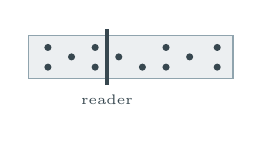
\begin{tikzpicture}
  \draw[draw=nLine, fill=nFill] (0,0) rectangle (2.6,0.55);
  \foreach \x/\y in {0.25/0.15,0.25/0.4,0.55/0.28,0.85/0.15,0.85/0.4,1.15/0.28,1.45/0.15,1.75/0.4,1.75/0.15,2.05/0.28,2.4/0.15,2.4/0.4}
    {\fill[nInk] (\x,\y) circle (0.045);}
  \draw[nInk, very thick] (1.0,-0.08) -- (1.0,0.63);
  \node[font=\tiny, text=nInk, anchor=north] at (1.0,-0.08) {reader};
\end{tikzpicture}}

\newcommand{\diagMemStackSmall}{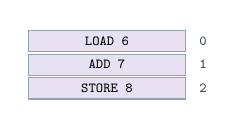
\begin{tikzpicture}
  \node[smallcell, fill=sViolet!18, minimum width=2.0cm] at (0,0.3) {LOAD 6};
  \node[smallcell, fill=sViolet!18, minimum width=2.0cm] at (0,0) {ADD 7};
  \node[smallcell, fill=sViolet!18, minimum width=2.0cm] at (0,-0.3) {STORE 8};
  \node[addr, font=\ttfamily\tiny, anchor=west] at (1.05,0.3) {0};
  \node[addr, font=\ttfamily\tiny, anchor=west] at (1.05,0) {1};
  \node[addr, font=\ttfamily\tiny, anchor=west] at (1.05,-0.3) {2};
\end{tikzpicture}}

\newcommand{\diagTwoMem}{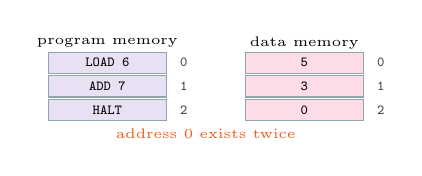
\begin{tikzpicture}
  \node[font=\tiny] at (0,0.55) {program memory};
  \node[font=\tiny] at (2.5,0.55) {data memory};
  \node[smallcell, fill=sViolet!18, minimum width=1.5cm] at (0,0.3) {LOAD 6};
  \node[smallcell, fill=sViolet!18, minimum width=1.5cm] at (0,0) {ADD 7};
  \node[smallcell, fill=sViolet!18, minimum width=1.5cm] at (0,-0.3) {HALT};
  \node[smallcell, fill=sPink!18, minimum width=1.5cm] at (2.5,0.3) {5};
  \node[smallcell, fill=sPink!18, minimum width=1.5cm] at (2.5,0) {3};
  \node[smallcell, fill=sPink!18, minimum width=1.5cm] at (2.5,-0.3) {0};
  \foreach \i in {0,1,2} {
    \node[addr, font=\ttfamily\tiny, anchor=west] at (0.8,{0.3-0.3*\i}) {\i};
    \node[addr, font=\ttfamily\tiny, anchor=west] at (3.3,{0.3-0.3*\i}) {\i};
  }
  \node[font=\tiny, text=AccentOrange] at (1.25,-0.6) {address 0 exists twice};
\end{tikzpicture}}

\newcommand{\diagOneMem}{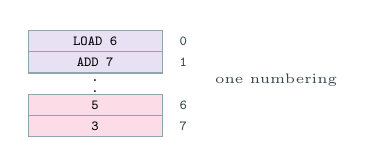
\begin{tikzpicture}
  \node[smallcell, fill=sViolet!18, minimum width=1.7cm] (o0) at (0,0.5) {LOAD 6};
  \node[smallcell, fill=sViolet!18, minimum width=1.7cm] at (0,0.23) {ADD 7};
  \node[smallcell, draw=none, minimum width=1.7cm] at (0,-0.04) {$\vdots$};
  \node[smallcell, fill=sPink!18, minimum width=1.7cm] at (0,-0.31) {5};
  \node[smallcell, fill=sPink!18, minimum width=1.7cm] at (0,-0.58) {3};
  \node[addr, font=\ttfamily\tiny, anchor=west] at (0.95,0.5) {0};
  \node[addr, font=\ttfamily\tiny, anchor=west] at (0.95,0.23) {1};
  \node[addr, font=\ttfamily\tiny, anchor=west] at (0.95,-0.31) {6};
  \node[addr, font=\ttfamily\tiny, anchor=west] at (0.95,-0.58) {7};
  \node[font=\tiny, text=nInk, anchor=west] at (1.4,0) {one numbering};
\end{tikzpicture}}

\newcommand{\diagDecimal}{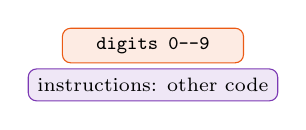
\begin{tikzpicture}
  \node[draw=AccentOrange, fill=AccentOrange!12, rounded corners=3pt, font=\ttfamily\scriptsize, minimum height=0.4cm,
    minimum width=2.3cm] at (0,0.28) {digits 0--9};
  \node[draw=ProgramPurple, fill=ProgramPurple!12, rounded corners=3pt, font=\scriptsize, minimum height=0.4cm,
    minimum width=2.3cm] at (0,-0.22) {instructions: other code};
\end{tikzpicture}}

\newcommand{\diagBinary}{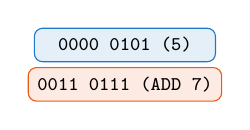
\begin{tikzpicture}
  \node[draw=StorageBlue, fill=StorageBlue!12, rounded corners=3pt, font=\ttfamily\scriptsize, minimum height=0.4cm,
    minimum width=2.3cm] at (0,0.28) {0000 0101 (5)};
  \node[draw=AccentOrange, fill=AccentOrange!12, rounded corners=3pt, font=\ttfamily\scriptsize, minimum height=0.4cm,
    minimum width=2.3cm] at (0,-0.22) {0011 0111 (ADD 7)};
\end{tikzpicture}}

\newcommand{\diagParallel}{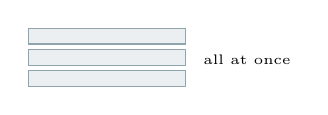
\begin{tikzpicture}
  \foreach \k in {0,1,2} {\draw[fill=nFill, draw=nLine] (0,{0.6-0.27*\k}) rectangle (2.0,{0.4-0.27*\k});}
  \node[font=\tiny, anchor=west] at (2.1,0.2) {all at once};
\end{tikzpicture}}

\newcommand{\diagDataflow}{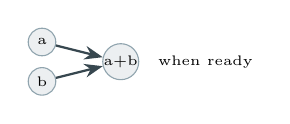
\begin{tikzpicture}[>=Stealth]
  \node[circle, draw=nLine, fill=nFill, minimum size=0.35cm, inner sep=0pt, font=\tiny] (a) at (0,0.3) {a};
  \node[circle, draw=nLine, fill=nFill, minimum size=0.35cm, inner sep=0pt, font=\tiny] (b) at (0,-0.2) {b};
  \node[circle, draw=nLine, fill=nFill, minimum size=0.4cm, inner sep=0pt, font=\tiny] (c) at (1.0,0.05) {a+b};
  \draw[->, thick, nInk] (a) -- (c); \draw[->, thick, nInk] (b) -- (c);
  \node[font=\tiny, anchor=west] at (1.35,0.05) {when ready};
\end{tikzpicture}}

\newcommand{\diagSequential}{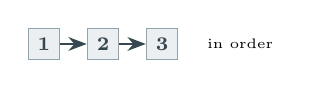
\begin{tikzpicture}[>=Stealth]
  \foreach \k in {1,2,3} {\node[draw=nLine, fill=nFill, text=nInk, minimum size=0.4cm, inner sep=0pt, font=\scriptsize\bfseries]
    (s\k) at ({0.75*\k-0.75},0.05) {\k};}
  \draw[->, thick, nInk] (s1) -- (s2); \draw[->, thick, nInk] (s2) -- (s3);
  \node[font=\tiny, anchor=west] at (1.95,0.05) {in order};
\end{tikzpicture}}

\newcommand{\diagMonolith}{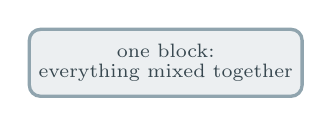
\begin{tikzpicture}
  \node[draw=nLine, very thick, rounded corners=4pt, fill=nFill, text=nInk, minimum width=2.6cm, minimum height=0.85cm,
    font=\scriptsize, align=center] {one block:\\[-1pt]everything mixed together};
\end{tikzpicture}}

\newcommand{\diagUnits}{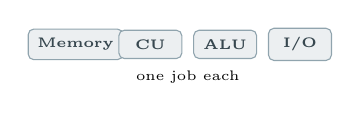
\begin{tikzpicture}
  \node[draw=nLine, fill=nFill, text=nInk, rounded corners=2pt, font=\tiny\bfseries, minimum width=0.8cm, minimum height=0.36cm] at (0,0.22) {Memory};
  \node[draw=nLine, fill=nFill, text=nInk, rounded corners=2pt, font=\tiny\bfseries, minimum width=0.8cm, minimum height=0.36cm] at (0.95,0.22) {CU};
  \node[draw=nLine, fill=nFill, text=nInk, rounded corners=2pt, font=\tiny\bfseries, minimum width=0.8cm, minimum height=0.36cm] at (1.9,0.22) {ALU};
  \node[draw=nLine, fill=nFill, text=nInk, rounded corners=2pt, font=\tiny\bfseries, minimum width=0.8cm, minimum height=0.36cm] at (2.85,0.22) {I/O};
  \node[font=\tiny] at (1.425,-0.2) {one job each};
\end{tikzpicture}}

% ---------- helpers for the CPU section ----------
\tikzset{
  reg/.style={draw=nLine, very thick, fill=white, text=nInk, rounded corners=2pt,
    minimum width=1.95cm, minimum height=0.55cm, inner sep=2pt, font=\ttfamily\scriptsize, align=center},
  cpuunit/.style={very thick, rounded corners=3pt, minimum width=1.2cm, minimum height=0.6cm,
    inner sep=2pt, font=\scriptsize\bfseries, align=center},
  hot/.style={aexec, label={[text=aExec, inner sep=1pt, font=\tiny]right:$\blacktriangleleft$}},
  hotdata/.style={aread},
  hotwrite/.style={awrite},
  hotalu/.style={aexec},
  fetcharrow/.style={-{Stealth}, very thick, DeepBlue, rounded corners=3pt},
  dataarrow/.style={-{Stealth}, very thick, DeepBlue, rounded corners=3pt},
  steplabel/.style={font=\tiny\bfseries, fill=white, inner sep=1pt},
}
% memory with the running example
% #1 highlighted instruction (0-3, -1 = none)  #2 text of cell 8  #3 highlighted data cell (6-8, 0 = none)
\newcommand{\mempanel}[3]{%
  \node[font=\scriptsize\bfseries, text=nInk] at (0,1.8) {Memory};
  \foreach \i/\t in {0/{0001 0110\ \ LOAD 6},1/{0011 0111\ \ ADD 7},2/{0010 1000\ \ STORE 8},3/{0111 0000\ \ HALT}} {
    \ifnum\i=#1
      \node[instrcell, minimum width=2.9cm, hot] (m\i) at (0,{1.35-0.45*\i}) {\t};
    \else
      \node[instrcell, minimum width=2.9cm] (m\i) at (0,{1.35-0.45*\i}) {\t};
    \fi
    \node[addr, anchor=east] at (-1.5,{1.35-0.45*\i}) {\i};
  }
  \node[memcell, draw=none, minimum width=2.9cm] at (0,-0.45) {$\vdots$};
  \foreach \i/\t/\y in {6/{0000 0101\ \ (5)}/-0.9,7/{0000 0011\ \ (3)}/-1.35,8/{#2}/-1.8} {
    \ifnum\i=#3
      \ifnum\i=8 \node[datacell, minimum width=2.9cm, hotwrite] (m\i) at (0,\y) {\t};\else \node[datacell, minimum width=2.9cm, hotdata] (m\i) at (0,\y) {\t};\fi
    \else
      \node[datacell, minimum width=2.9cm] (m\i) at (0,\y) {\t};
    \fi
    \node[addr, anchor=east] at (-1.5,\y) {\i};
  }
}
% the CPU, built up step by step
% #1 level: 0 empty, 1 +PC, 2 +IR, 3 +AC, 4 +ALU, 5 +CU   #2 PC   #3 IR   #4 AC   #5 extra ALU style
\newcommand{\cpupanel}[5]{%
  \node[draw=nLine, very thick, rounded corners=6pt, fill=nFill!50, minimum width=4.65cm,
    minimum height=3.85cm, anchor=west] (cpu) at (2.45,-0.2) {};
  \node[font=\scriptsize\bfseries, text=nInk, anchor=north west] at ([shift={(0.1,-0.06)}]cpu.north west) {CPU};
  \ifnum#1>0 \node[reg] (pc) at (3.65,0.95) {\textbf{PC}\ \ #2}; \fi
  \ifnum#1>1 \node[reg] (ir) at (3.65,0.0) {\textbf{IR}\\[-1pt]#3}; \fi
  \ifnum#1>2 \node[reg] (ac) at (3.65,-1.05) {\textbf{AC}\ \ #4}; \fi
  \ifnum#1>3 \node[cpuunit, draw=mygreen, fill=mygreen!18, #5] (alu) at (6.3,-1.05)
    {\textcolor{mygreen!60!black}{\faCalculator}\\[-1pt]ALU}; \fi
  \ifnum#1>4 \node[cpuunit, draw=AccentOrange, fill=AccentOrange!18] (cu) at (6.3,0.5)
    {\textcolor{AccentOrange}{\faCogs}\\[-1pt]CU}; \fi
}
% explanation slide: #1 title, #2 tikz body (memory + CPU), #3 right-hand column
\newcommand{\explainframe}[3]{%
\begin{frame}{#1}
  \begin{columns}[c,onlytextwidth]
    \column{0.58\textwidth}
      \centering
      \begin{tikzpicture}[>=Stealth, scale=0.92, every node/.append style={transform shape}]
        #2
      \end{tikzpicture}
    \column{0.4\textwidth}
      #3
  \end{columns}
\end{frame}}
% boxes for the right-hand column
\newcommand{\defbox}[1]{%
  \begin{beamercolorbox}[rounded=true,sep=0.1cm,wd=\linewidth]{block body example}
    \footnotesize #1
  \end{beamercolorbox}\vspace{0.06cm}}
\newcommand{\stepbox}[2]{%
  \begin{beamercolorbox}[rounded=true,sep=0.09cm,wd=\linewidth]{block body}
    \footnotesize\textbf{#1}\\ #2
  \end{beamercolorbox}\vspace{0.06cm}}
\newcommand{\phasename}[1]{%
  {\centering\footnotesize Name of this phase:\ \colorbox{DeepBlue}{\textcolor{white}{\textbf{#1}}}\par}}
% small tag above the CPU box: which instruction is being executed
\newcommand{\executing}[1]{%
  \node[font=\scriptsize\bfseries, text=AccentOrange, anchor=south east] at ([yshift=1pt]cpu.north east)
    {Executing: \texttt{#1}};}
\newcommand{\statebox}[1]{%
  {\centering\scriptsize\textcolor{DeepBlue}{\textbf{State:}}\ #1\par}}

\lstset{
  language=Python,
  basicstyle=\color{VSText}\ttfamily\footnotesize,
  keywordstyle=\color{VSPurple}\bfseries,
  stringstyle=\color{VSString},
  commentstyle=\color{VSComment}\itshape,
  numbers=left,
  numberstyle=\tiny\color{gray},
  stepnumber=1,
  breaklines=true,
  showstringspaces=false,
  xleftmargin=15pt,
  xrightmargin=5pt,
  frame=none
}

% MARIE assembly: line numbers start at 0, so a line number equals the memory address
\lstdefinelanguage{MARIE}{
  morekeywords={Load,Store,Add,Subt,Input,Output,Halt,Jump,Skipcond,DEC,HEX,ADR,LoadI,StoreI,AddI,JumpI,JnS,Clear,LoadImmi},
  sensitive=false,
  comment=[l]{/},
}
\lstdefinestyle{marie}{language=MARIE, firstnumber=0, basicstyle=\color{VSText}\ttfamily\scriptsize,
  keywordstyle=\color{VSBlue}\bfseries, commentstyle=\color{VSComment}\itshape,
  columns=fixed, basewidth=0.52em, keepspaces=true, breaklines=false, xleftmargin=12pt}

\BeforeBeginEnvironment{lstlisting}{%
  \begin{beamercolorbox}[rounded=true,sep=2mm,wd=\linewidth]{vscodelisting}%
  
\begin{tikzpicture}
    \fill[nLine] (0,0) circle (3pt);
    \fill[nLine] (0.35,0) circle (3pt);
    \fill[nLine] (0.70,0) circle (3pt);
  \end{tikzpicture}%
  \vspace{-0.2cm}%
}
\AfterEndEnvironment{lstlisting}{\end{beamercolorbox}}

% =====================================================================
%  Day 2 helpers
% =====================================================================

% ---------- MARIE datapath, drawn like the Data Path view of MARIE.js ----------
% \busdiagram[values]{source}{destination}{extra TikZ}
%   source (Read, blue) and destination (Write, red): ir, out, in, ac, mbr, pc, mar, mem, none
%   values: ir=, out=, in=, ac=, mbr=, pc=, mar=, mem= (contents of M[MAR]), step= (0-7, -1 = none)
\definecolor{ReadBlue}{HTML}{1E88E5}
\definecolor{WriteRed}{HTML}{E53935}
\definecolor{BusGreen}{HTML}{B0BEC5}% the bus: neutral
\tikzset{
  dpreg/.style={draw=nLine, thick, fill=white, text=nInk, minimum width=1.1cm, minimum height=0.46cm,
    inner sep=1pt, font=\ttfamily\scriptsize},
  dpname/.style={font=\tiny, text=nInk, above=0pt, inner sep=1pt},
  dpwire/.style={thin, nLight},
  dpmem/.style={draw=nLine, very thick, fill=nFill, rounded corners=3pt,
    minimum width=1.3cm, minimum height=0.95cm, font=\scriptsize\bfseries, align=center},
  srcreg/.style={draw=ReadBlue, line width=1.6pt},
  dstreg/.style={draw=WriteRed, line width=1.6pt},
}
\pgfkeys{/dp/.is family, /dp,
  ir/.initial={0000}, out/.initial={0000}, in/.initial={0000}, ac/.initial={0000},
  mbr/.initial={0000}, pc/.initial={000}, mar/.initial={000}, mem/.initial={0000},
  step/.initial={-1}}
\newcommand{\dpv}[1]{\pgfkeysvalueof{/dp/#1}}
\newcommand{\busdiagram}[4][]{%
  \begingroup
  \pgfkeys{/dp, ir=0000, out=0000, in=0000, ac=0000, mbr=0000, pc=000, mar=000, mem=0000, step=-1, #1}%
  \begin{tikzpicture}[>=Stealth]
    \tikzset{bd-mem/.style={}, bd-mar/.style={}, bd-pc/.style={}, bd-mbr/.style={},
      bd-ac/.style={}, bd-ir/.style={}, bd-in/.style={}, bd-out/.style={}, bd-none/.style={}}
    \tikzset{bd-#2/.style={srcreg}}
    \tikzset{bd-#3/.style={dstreg}}
    % ----- control unit -----
    \node[draw=DeepBlue!80, thick, fill=white, minimum width=1.3cm, minimum height=2.95cm,
      anchor=north west] (cu) at (-2.4,2.0) {};
    \node[font=\tiny, text=DeepBlue, anchor=north west, below=1pt] at (cu.south west) {Control unit};
    \node[font=\tiny, text=DeepBlue!80, anchor=east] at (-1.15,1.75) {Read};
    \node[font=\tiny, text=DeepBlue!80, anchor=east] at (-1.15,-0.6) {Write};
    \node[font=\tiny, text=DeepBlue!80, anchor=east] at (-1.15,0.05) {AC<0};
    \node[font=\tiny, text=DeepBlue!80, anchor=east] at (-1.15,-0.15) {AC=0};
    \node[font=\tiny, text=DeepBlue!80] at (-2.0,1.3) {Step};
    \foreach \k in {0,...,7} {
      \pgfmathtruncatemacro{\cur}{\dpv{step}}
      \ifnum\k=\cur
        \fill[AccentOrange] (-2.0,{1.1-0.15*\k}) circle (0.065);
      \else
        \fill[DeepBlue!30] (-2.0,{1.1-0.15*\k}) circle (0.035);
      \fi
    }
    % ----- memory -----
    \node[draw=DeepBlue!80, thick, fill=white, minimum width=1.5cm, minimum height=2.95cm,
      anchor=north west, bd-mem] (mem) at (10.4,2.0) {};
    \node[font=\tiny, text=DeepBlue, anchor=north west, below=1pt] at (mem.south west) {Main memory};
    \node[font=\ttfamily\tiny, text=DeepBlue!80] at (11.15,0.75) {M[MAR]};
    \node[font=\ttfamily\scriptsize] at (11.15,0.5) {\dpv{mem}};
    % ----- faint control wires (one Read and one Write wire per device) -----
    \draw[dpwire] (-1.1,1.75) -- (10.4,1.75);
    \draw[dpwire] (-1.1,-0.6) -- (10.4,-0.6);
    \foreach \x in {0.6,2.0,3.4,4.8,6.2,7.6,9.0} {
      \draw[dpwire] (\x-0.25,1.75) -- (\x-0.25,1.18);
      \draw[dpwire] (\x+0.3,-0.6) -- (\x+0.3,0.72);
    }
    % ----- bus (drawn first, registers on top) -----
    \foreach \x in {0.6,2.0,3.4,4.8,6.2,7.6,9.0}
      \draw[line width=2.6pt, BusGreen] (\x,0.72) -- (\x,-0.35);
    \draw[line width=2.6pt, BusGreen] (0.6-0.045,-0.35) -- (10.4,-0.35);
    % ----- ALU between AC and MBR, with its links and the flag wires to the CU -----
    \draw[thin, DeepBlue!40] (4.45,0.05) -- (-1.1,0.05);
    \draw[thin, DeepBlue!40] (4.45,-0.15) -- (-1.1,-0.15);
    \draw[thick, DeepBlue!70, fill=white] (5.0,0.47) -- (5.42,0.47) -- (5.5,0.37) -- (5.58,0.47) -- (6.0,0.47)
      -- (5.72,0.05) -- (5.28,0.05) -- cycle;
    \node[font=\tiny, text=DeepBlue!80] at (5.5,0.22) {ALU};
    \draw[thick, DeepBlue!60] (5.2,0.72) -- (5.2,0.47);
    \draw[thick, DeepBlue!60] (5.8,0.72) -- (5.8,0.47);
    \draw[thick, DeepBlue!60] (5.5,0.05) -- (5.5,-0.1) -- (4.45,-0.1) |- (4.45,0.72);
    % ----- registers -----
    \foreach \n/\x/\lab in {ir/0.6/IR, out/2.0/OUT, in/3.4/IN, ac/4.8/AC, mbr/6.2/MBR, pc/7.6/PC, mar/9.0/MAR} {
      \node[dpreg, bd-\n] (\n) at (\x,0.95) {\dpv{\n}};
      \node[dpname] at (\n.north) {\lab};
      \coordinate (\n-port) at (\n.south);
      \coordinate (\n-bus) at (\x,-0.35);
    }
    \coordinate (mem-port) at (10.4,-0.35);
    \coordinate (mem-bus) at (10.4,-0.35);
    % IR is decoded by the CU; MAR selects the memory cell
    \draw[thick, BusGreen, -{Stealth}] (ir.west) -- (-1.1,0.95);
    \draw[thick, BusGreen, -{Stealth}] (mar.east) -- (10.4,0.95);
    % ----- active Read and Write signals -----
    \ifstrequal{#2}{none}{}{%
      \ifstrequal{#2}{mem}
        {\draw[line width=1.3pt, ReadBlue, -{Stealth}] (-1.1,1.75) -- (10.4,1.75);}
        {\draw[line width=1.3pt, ReadBlue, -{Stealth}] (-1.1,1.75) -| ($(#2.north)+(-0.25,0)$);}}
    \ifstrequal{#3}{none}{}{%
      \ifstrequal{#3}{mem}
        {\draw[line width=1.3pt, WriteRed, -{Stealth}] (-1.1,-0.6) -- (10.4,-0.6);}
        {\draw[line width=1.3pt, WriteRed, -{Stealth}] (-1.1,-0.6) -| ($(#3.south)+(0.3,0)$);}}
    % ----- the value travelling along the bus -----
    \ifstrequal{#2}{none}{}{\ifstrequal{#3}{none}{}{%
      \draw[line width=3pt, nInk] (#2-port) -- (#2-bus) -- (#3-bus) -- (#3-port);
      \draw[line width=1.5pt, white, dash pattern=on 1.5pt off 1.5pt] (#2-port) -- (#2-bus) -- (#3-bus) -- (#3-port);}}
    #4
  \end{tikzpicture}%
  \endgroup}

% legend for the colours of the data path
\newcommand{\dplegend}{%
  {\tiny\textcolor{ReadBlue}{\rule{0.25cm}{0.2cm}}\ \textbf{Read}: puts its value on the bus
  \qquad\textcolor{WriteRed}{\rule{0.25cm}{0.2cm}}\ \textbf{Write}: stores the value from the bus
  \qquad\tikz[baseline=-0.6ex]{\draw[line width=3pt, BusGreen] (0,0) -- (0.5,0);\draw[line width=1.5pt, white, dash pattern=on 1.5pt off 1.5pt] (0,0) -- (0.5,0);}\ the value travelling on the bus}}

% one step of an instruction: data path on top, explanation below
% #1 title, #2 source, #3 destination, #4 values (keys), #5 explanation
\newcommand{\stepframe}[5]{%
\begin{frame}{#1}
  \begin{center}
    \resizebox{0.8\textwidth}{!}{\busdiagram[#4]{#2}{#3}{}}\\[0.02cm]
    \dplegend
  \end{center}
  \vspace{-0.1cm}
  \begin{center}
    \begin{minipage}{0.8\textwidth}
      #5
    \end{minipage}
  \end{center}
\end{frame}}

% ---------- timeline of clock steps ----------
% #1 fetch steps, #2 execute steps, #3 label on the right
\newcommand{\steptimeline}[3]{%
  \begin{tikzpicture}
    \foreach \i in {1,...,#1}
      \node[draw=white, fill=sAmber, text=black, font=\tiny\bfseries, minimum width=0.62cm,
        minimum height=0.45cm, inner sep=0pt] at ({0.62*(\i-1)},0) {T\the\numexpr\i-1\relax};
    \foreach \i in {1,...,#2}
      \node[draw=white, fill=sTeal, text=white, font=\tiny\bfseries, minimum width=0.62cm,
        minimum height=0.45cm, inner sep=0pt] at ({0.62*(#1+\i-1)},0) {T\the\numexpr#1+\i-1\relax};
    \node[anchor=west, font=\scriptsize] at ({0.62*(#1+#2)-0.25},0) {#3};
  \end{tikzpicture}}

% legend for the timeline colours
\newcommand{\timelinelegend}{%
  {\tiny\textcolor{StorageBlue!75}{\rule{0.25cm}{0.2cm}}\ fetch
  \qquad\textcolor{AccentOrange}{\rule{0.25cm}{0.2cm}}\ execute}}

% ---------- small pieces for the addressing-mode slides ----------
\tikzset{
  mcell/.style={draw=DeepBlue!60, minimum width=1.5cm, minimum height=0.42cm, inner sep=1pt,
    font=\ttfamily\scriptsize, align=center, fill=StorageBlue!15},
  mcellhot/.style={mcell, fill=StorageBlue!45, draw=StorageBlue, very thick},
  mcellptr/.style={mcell, fill=ProgramPurple!18, draw=ProgramPurple, very thick},
  instrbox/.style={draw=AccentOrange, very thick, fill=AccentOrange!15, rounded corners=2pt,
    minimum height=0.5cm, inner sep=3pt, font=\ttfamily\scriptsize},
  ptrarrow/.style={-{Stealth}, very thick, DeepBlue},
  valarrow/.style={-{Stealth}, very thick, DeepBlue},
}

% task header box (same look as on Day 1)
% #1 form and time, #2 short instruction
\newcommand{\taskhead}[2]{%
  \begin{beamercolorbox}[rounded=true,sep=0.12cm,wd=\linewidth]{block body example}
    \small\textbf{#1}\\[0.04cm]
    \footnotesize #2
  \end{beamercolorbox}\vspace{0.1cm}}

% highlighted key message at the bottom of a slide
\newcommand{\keymsg}[1]{%
  \begin{beamercolorbox}[rounded=true,sep=0.1cm,wd=\textwidth]{block body example}
    \centering\footnotesize #1
  \end{beamercolorbox}}

% register transfer written in text: \mo{MAR}{PC} gives MAR <- PC
\newcommand{\mo}[2]{\texttt{#1\,$\leftarrow$\,#2}}

% plain listings (x86, RISC-V) without Python highlighting
\lstdefinelanguage{plain}{}
\lstdefinestyle{asm}{language=plain, basicstyle=\color{VSText}\ttfamily\scriptsize, numbers=none,
  columns=fixed, basewidth=0.52em, keepspaces=true, xleftmargin=6pt}

% =====================================================================
%  Day 3 helpers
% =====================================================================

\usetikzlibrary{patterns}
\usepackage{multirow}
% ---------- RISC-V listings ----------
\lstdefinestyle{rv}{language=RISCV, basicstyle=\color{VSText}\ttfamily\scriptsize, numbers=none,
  keywordstyle=\color{VSBlue}\bfseries, keywordstyle={[2]\color{VSPurple}\bfseries},
  commentstyle=\color{VSComment}\itshape,
  columns=fixed, basewidth=0.52em, keepspaces=true, breaklines=false, xleftmargin=6pt}
\lstdefinestyle{rvnum}{style=rv, numbers=left, firstnumber=1, xleftmargin=14pt}

% ---------- colours of the five pipeline stages (the same all day) ----------
\colorlet{cIF}{sAmber}
\colorlet{cID}{sBrown}
\colorlet{cEX}{sTeal}
\colorlet{cMEM}{sIndigo}
\colorlet{cWB}{sPink}
% text on a stage colour (amber needs black)
\colorlet{txIF}{black}\colorlet{txID}{white}\colorlet{txEX}{white}\colorlet{txMEM}{white}\colorlet{txWB}{white}
\colorlet{txcIF}{black}\colorlet{txcID}{white}\colorlet{txcEX}{white}\colorlet{txcMEM}{white}\colorlet{txcWB}{white}

% ---------- pipeline diagrams ----------
% cell size (cm)
\def\pw{0.74}
\def\ph{0.46}
\tikzset{
  pcell/.style={minimum width=\pw cm, minimum height=\ph cm, inner sep=0pt, draw=white,
    font=\scriptsize\bfseries, text=white},
  pst-IF/.style={pcell, fill=cIF, text=black},
  pst-ID/.style={pcell, fill=cID},
  pst-EX/.style={pcell, fill=cEX},
  pst-MEM/.style={pcell, fill=cMEM},
  pst-WB/.style={pcell, fill=cWB},
  pst-B/.style={pcell, fill=nIdle, text=nInk, font=\tiny},
  pst-X/.style={pcell, fill=nFill, text=nInk, draw=nLine},
  pst-N/.style={pcell, fill=none, draw=none},
  pst-E/.style={pcell, fill=nFill!60},
  plab/.style={anchor=east, font=\ttfamily\footnotesize, inner sep=1pt},
}
% one row of a pipeline diagram
% #1 row (0 = top), #2 first cycle (1-based), #3 comma list of IF, ID, EX, MEM, WB, B (bubble), X (flushed), N (empty)
\newcommand{\prow}[3]{%
  \foreach \s [count=\k from 0] in {#3} {%
    \node[pst-\s] at ({(#2+\k-1)*\pw}, {-(#1)*\ph}) {%
      \expandafter\ifstrequal\expandafter{\s}{B}{bubble}{%
      \expandafter\ifstrequal\expandafter{\s}{X}{$\times$}{%
      \expandafter\ifstrequal\expandafter{\s}{N}{}{\expandafter\ifstrequal\expandafter{\s}{E}{}{\s}}}}};
  }}
% label of a row
\newcommand{\plabel}[2]{\node[plab] at ({-0.5*\pw-0.05}, {-(#1)*\ph}) {#2};}
% cycle numbers above the diagram: #1 number of cycles
\newcommand{\pcycles}[1]{%
  \foreach \c in {1,...,#1}
    \node[font=\scriptsize, text=DeepBlue!70] at ({(\c-1)*\pw}, {0.8*\ph}) {\c};
  \node[font=\scriptsize, text=DeepBlue!70, anchor=east] at ({-0.5*\pw-0.05}, {0.8*\ph}) {cycle};}
% highlight one column: #1 cycle, #2 number of rows, #3 colour
\newcommand{\pcolumn}[3]{%
  \draw[#3, very thick, rounded corners=2pt]
    ({(#1-1.5)*\pw}, {0.5*\ph}) rectangle ({(#1-0.5)*\pw}, {-(#2-0.5)*\ph});}

% legend of stage colours
\newcommand{\stagelegend}{%
  {\tiny
  \textcolor{cIF}{\rule{0.25cm}{0.2cm}}\,IF fetch\quad
  \textcolor{cID}{\rule{0.25cm}{0.2cm}}\,ID decode\quad
  \textcolor{cEX}{\rule{0.25cm}{0.2cm}}\,EX execute\quad
  \textcolor{cMEM}{\rule{0.25cm}{0.2cm}}\,MEM memory\quad
  \textcolor{cWB}{\rule{0.25cm}{0.2cm}}\,WB write back}}

% ---------- stage boxes ----------
\tikzset{
  stagebox/.style={very thick, rounded corners=4pt, minimum width=1.9cm, minimum height=0.8cm,
    align=center, font=\small\bfseries, drop shadow},
  gbar/.style={minimum height=0.36cm, inner sep=0pt, draw=white, font=\tiny\bfseries, text=white},
  gempty/.style={minimum height=0.36cm, inner sep=0pt, draw=gray!50, dashed, font=\tiny, text=gray!60},
  unit/.style={draw=nLine, very thick, fill=white, text=nInk, rounded corners=3pt, align=center,
    font=\scriptsize\bfseries, inner sep=2pt},
}

% ---------- a simple RISC-V datapath ----------
% #1 extra TikZ drawn on top (nodes: pc, imem, rf, alu, dmem, mux, cu, add4)
\newcommand{\rvdatapath}[1]{%
  \begin{tikzpicture}[>=Stealth, font=\scriptsize]
    % stage labels
    \foreach \x/\n/\c in {0.9/IF/cIF, 4.2/ID/cID, 6.6/EX/cEX, 9.0/MEM/cMEM, 10.9/WB/cWB}
      \node[fill=\c, text=tx\c, rounded corners=2pt, font=\tiny\bfseries, minimum width=0.9cm] at (\x,2.35) {\n};
    % units
    \node[unit, minimum width=0.6cm, minimum height=1.0cm] (pc) at (0,0) {PC};
    \node[unit, minimum width=1.5cm, minimum height=1.6cm] (imem) at (1.8,0) {Instruction\\memory};
    \node[unit, minimum width=1.5cm, minimum height=1.8cm] (rf) at (4.2,0) {Register\\file};
    \draw[nInk, very thick, fill=white] (6.2,0.9) -- (7.0,0.45) -- (7.0,-0.45) -- (6.2,-0.9) -- (6.2,-0.25)
      -- (6.4,0) -- (6.2,0.25) -- cycle;
    \node[font=\scriptsize\bfseries] (alu) at (6.68,0) {ALU};
    \coordinate (aluin1) at (6.2,0.55); \coordinate (aluin2) at (6.2,-0.55); \coordinate (aluout) at (7.0,0);
    \node[unit, minimum width=1.5cm, minimum height=1.6cm] (dmem) at (9.0,0) {Data\\memory};
    \node[unit, minimum width=0.45cm, minimum height=1.2cm, rounded corners=6pt, font=\tiny] (mux) at (10.9,0) {M\\U\\X};
    \node[unit, minimum width=1.3cm, minimum height=0.5cm, draw=nLine, text=nLine] (add4) at (0.9,1.55) {$+4$};
    \node[unit, minimum width=2.2cm, minimum height=0.5cm, draw=gray, text=gray] (cu) at (4.2,-1.85) {Control unit};
    % wires
    \draw[->, thick] (pc) -- (imem);
    \draw[->, thick] (imem) -- node[above, font=\tiny] {instruction} (rf);
    \draw[->, thick] ([yshift=0.55cm]rf.east) -- (aluin1);
    \draw[->, thick] ([yshift=-0.55cm]rf.east) -- (aluin2);
    \draw[->, thick] (aluout) -- node[above, font=\tiny] {address} ([yshift=0cm]dmem.west);
    \draw[->, thick] ([yshift=-0.55cm]dmem.east) -- ([yshift=-0.4cm]mux.west);
    \draw[->, thick] (7.3,0) |- (7.3,-1.1) -| (10.3,-1.1) |- ([yshift=0.4cm]mux.west);
    \draw[->, thick] (mux.east) -- ++(0.3,0) |- (11.2,2.0) -| node[pos=0.25, above, font=\tiny] {write back} (4.2,0.9);
    \draw[->, thick, nLine] (pc.north) |- (add4.west);
    \draw[->, thick, nLine] (add4.east) -- ++(0.35,0) |- (-0.6,1.95) |- (pc.west);
    \draw[->, dashed, gray] (cu.north) -- (rf.south);
    \draw[->, dashed, gray] (cu.east) -| (dmem.south);
    \draw[->, dashed, gray] (cu.east) -| (mux.south);
    #1
  \end{tikzpicture}}

% ---------- Ripes window (schematic; replace with a real screenshot if you like) ----------
\newcommand{\ripeswindow}{%
  \begin{tikzpicture}[font=\tiny]
    \draw[nInk, very thick, fill=white, rounded corners=4pt] (0,0) rectangle (9,5.4);
    \fill[nLight, rounded corners=4pt] (0,5.0) rectangle (9,5.4);
    \fill[MacRed] (0.25,5.2) circle (2.5pt); \fill[MacYellow] (0.5,5.2) circle (2.5pt); \fill[MacGreen] (0.75,5.2) circle (2.5pt);
    \node[font=\tiny\bfseries, text=nInk] at (4.5,5.2) {Ripes};
    % toolbar
    \fill[LightGray] (0,4.55) rectangle (9,5.0);
    \foreach \x/\i in {1.0/\faMicrochip, 1.6/\faStepForward, 2.2/\faPlay, 2.8/\faFastForward, 3.4/\faUndo}
      \node[text=nInk] at (\x,4.77) {\i};
    % side bar
    \fill[nLine] (0,0) rectangle (0.5,4.55);
    \foreach \y/\i in {4.1/\faEdit, 3.5/\faMicrochip, 2.9/\faMemory, 2.3/\faTerminal}
      \node[text=white] at (0.25,\y) {\i};
    % editor
    \draw[gray!60, fill=VSDarkBg] (0.65,0.15) rectangle (3.2,4.4);
    \foreach \y/\t in {4.1/lw x5{,} X, 3.8/lw x6{,} Y, 3.5/add x7{,} x5{,} x6, 3.2/addi x7{,} x7{,} -2, 2.9/sw x7{,} Z{,} x28}
      \node[anchor=west, text=VSText, font=\ttfamily\tiny] at (0.75,\y) {\t};
    % processor view
    \draw[gray!60, fill=LightGray] (3.35,1.4) rectangle (7.3,4.4);
    \foreach \x/\c in {3.8/cIF, 4.5/cID, 5.3/cEX, 6.1/cMEM, 6.8/cWB}
      \draw[\c, very thick, fill=\c!15] (\x-0.25,2.3) rectangle (\x+0.25,3.6);
    \draw[->, thick, nLine] (3.55,2.95) -- (7.05,2.95);
    \node[font=\tiny, text=nInk] at (5.3,1.85) {datapath};
    % statistics
    \draw[gray!60, fill=white] (3.35,0.15) rectangle (7.3,1.25);
    \node[anchor=west, font=\tiny] at (3.45,0.95) {Cycles: 13};
    \node[anchor=west, font=\tiny] at (3.45,0.7) {Instrs. retired: 8};
    \node[anchor=west, font=\tiny] at (3.45,0.45) {CPI: 1.63 \quad IPC: 0.62};
    % registers
    \draw[gray!60, fill=white] (7.45,0.15) rectangle (8.85,4.4);
    \foreach \k [count=\j from 0] in {x5,x6,x7,x8,x9,x10}
      \node[anchor=west, font=\ttfamily\tiny] at (7.5,{4.1-0.3*\j}) {\k};
    \node[font=\tiny, text=nInk] at (8.15,2.1) {registers};
    % badges
    \node[circle, fill=AccentOrange, text=white, font=\bfseries\scriptsize, inner sep=1.5pt] at (1.9,1.2) {1};
    \node[circle, fill=AccentOrange, text=white, font=\bfseries\scriptsize, inner sep=1.5pt] at (1.35,4.77) {2};
    \node[circle, fill=AccentOrange, text=white, font=\bfseries\scriptsize, inner sep=1.5pt] at (5.3,4.1) {3};
    \node[circle, fill=AccentOrange, text=white, font=\bfseries\scriptsize, inner sep=1.5pt] at (6.95,0.7) {4};
    \node[circle, fill=AccentOrange, text=white, font=\bfseries\scriptsize, inner sep=1.5pt] at (8.15,1.4) {5};
  \end{tikzpicture}}

% small orange number used in running text
\newcommand{\badge}[1]{\tikz[baseline=(b.base)]\node[circle,fill=AccentOrange,text=white,
  inner sep=1.2pt,font=\bfseries\tiny] (b) {#1};}

% =====================================================================
%  Day 4 helpers
% =====================================================================

% ---------- colours of the memory levels (the same all day) ----------
% memory levels are hardware: neutral
\colorlet{cReg}{nInk}
\colorlet{cCache}{nInk}
\colorlet{cRAM}{nLine}
\colorlet{cDisk}{nLine}
\colorlet{cIO}{nInk}
\colorlet{HitGreen}{aExec}
\colorlet{MissRed}{aWrite}
\setbeamercolor{block body answer}{bg=aExec!8,fg=black}

% ---------- listings ----------
% RISC-V: the Day 3 keywords plus the new ones used today
\lstdefinelanguage{RISCV}{
  morekeywords={lw,sw,add,addi,sub,beq,bne,bnez,beqz,la,li,auipc,nop,ecall},
  morekeywords=[2]{.data,.text,.word,.zero},
  alsoletter={.},
  sensitive=true,
  morecomment=[l]{\#},
}
% C (for the locality examples)
\lstdefinestyle{cc}{language=C, basicstyle=\color{VSText}\ttfamily\scriptsize, numbers=none,
  keywordstyle=\color{VSBlue}\bfseries, commentstyle=\color{VSComment}\itshape,
  columns=fixed, basewidth=0.52em, keepspaces=true, breaklines=false, xleftmargin=6pt,
  moredelim=**[is][\color{MacYellow}\bfseries]{@}{@}}

% ---------- boxes for the memory levels and devices ----------
\tikzset{
  lbox/.style={very thick, rounded corners=4pt, align=center, font=\scriptsize\bfseries, inner sep=3pt},
  cpubox/.style={lbox, draw=nInk, fill=nInk, text=white},
  regbox/.style={lbox, draw=nLine, fill=nFill, text=nInk},
  cachebox/.style={lbox, draw=nLine, fill=nFill, text=nInk},
  rambox/.style={lbox, draw=nLine, fill=nFill, text=nInk},
  diskbox/.style={lbox, draw=nLine, fill=nFill, text=nInk},
  iobox/.style={lbox, draw=cIO, fill=cIO!12},
  dmabox/.style={lbox, draw=nLine, fill=nFill, text=nInk},
  osbox/.style={lbox, draw=nLine, fill=nFill, text=nInk},
  greybox/.style={lbox, draw=nLight, fill=white, text=nLine},
  arr/.style={-{Stealth}, very thick, nInk},
  okarr/.style={-{Stealth}, very thick, HitGreen},
  badarr/.style={-{Stealth}, very thick, MissRed},
  smalltxt/.style={font=\tiny, inner sep=1pt},
}

% ---------- design question box (as on the Day 1 dilemma slides) ----------
\newcommand{\designq}[1]{%
  \begin{beamercolorbox}[rounded=true,sep=0.14cm,wd=\textwidth]{block body}
    \centering\small\textbf{Design question:} #1
  \end{beamercolorbox}}
\newcommand{\whichone}{%
  {\centering\small\textcolor{DeepBlue}{\textbf{Which would you choose, and why?}}\par}}

% ---------- question card and answer card ----------
% #1 icon, #2 text
\newcommand{\qcard}[2]{%
  \begin{beamercolorbox}[rounded=true,sep=0.14cm,wd=\linewidth]{block body}
    \centering{\Large\textcolor{AccentOrange}{#1}}\\[0.12cm]
    \footnotesize #2
  \end{beamercolorbox}}
% #1 title, #2 text
\newcommand{\acard}[2]{%
  \begin{beamercolorbox}[rounded=true,sep=0.1cm,wd=\linewidth]{block body answer}
    \footnotesize\textbf{\textcolor{aExec}{\faCheck}\ #1}\\ #2
  \end{beamercolorbox}\vspace{0.06cm}}
% red "problem" box
\setbeamercolor{block body problem}{bg=AccentOrange!10,fg=black}
\newcommand{\probbox}[2]{%
  \begin{beamercolorbox}[rounded=true,sep=0.09cm,wd=\linewidth]{block body problem}
    \footnotesize\textbf{\textcolor{AccentOrange}{\faExclamationTriangle}\ #1}\\ #2
  \end{beamercolorbox}\vspace{0.06cm}}

% ---------- hits and misses ----------
\def\cw{0.62}
\def\chh{0.42}
\tikzset{
  hmcell/.style={minimum width=\cw cm, minimum height=\chh cm, inner sep=0pt, draw=white,
    font=\scriptsize\bfseries, text=white},
  hm-H/.style={hmcell, fill=white, draw=nLight, text=aExec},
  hm-M/.style={hmcell, fill=white, draw=nLight, text=aWrite},
  hm-Q/.style={hmcell, fill=nFill, draw=nLight, text=nLine},
  hm-A/.style={hmcell, draw=none, text=nInk, font=\scriptsize\ttfamily\bfseries},
}
% one row of hits and misses: #1 row (0 = top), #2 comma list of H, M, Q (Q = to fill in)
\newcommand{\hmrow}[2]{%
  \foreach \s [count=\k from 0] in {#2} {%
    \node[hm-\s] at ({\k*\cw}, {-(#1)*\chh}) {\expandafter\ifstrequal\expandafter{\s}{Q}{?}{\s}};}}
% the accessed addresses above a row: #1 row, #2 comma list
\newcommand{\hmhead}[2]{%
  \foreach \s [count=\k from 0] in {#2}
    \node[hm-A] at ({\k*\cw}, {-(#1)*\chh}) {\s};}
% label on the left of a row: #1 row, #2 text
\newcommand{\hmlabel}[2]{\node[anchor=east, font=\scriptsize, inner sep=1pt] at ({-0.5*\cw-0.08}, {-(#1)*\chh}) {#2};}
% label on the right of a row: #1 row, #2 number of cells, #3 text
\newcommand{\hmresult}[3]{\node[anchor=west, font=\scriptsize\bfseries, text=nInk, inner sep=1pt]
  at ({(#2-0.5)*\cw+0.12}, {-(#1)*\chh}) {#3};}

% ---------- a small cache (or page table) drawn as a table ----------
\tikzset{
  ctab/.style={draw=nLine, text=nInk, minimum height=0.4cm, inner sep=1pt, font=\ttfamily\scriptsize, fill=white},
  ctabh/.style={ctab, fill=nInk, text=white, font=\scriptsize\bfseries},
  ctabhit/.style={fill=HitGreen!25, draw=HitGreen, very thick},
  ctabmiss/.style={fill=MissRed!20, draw=MissRed, very thick},
}
% #1 comma list of line/valid/tag/data ; columns: Line, V, Tag, Data (top-left corner at the origin)
\newcommand{\cachetable}[1]{%
  \node[ctabh, minimum width=0.9cm] at (0,0) {Line};
  \node[ctabh, minimum width=0.7cm] at (0.8,0) {V};
  \node[ctabh, minimum width=1.0cm] at (1.65,0) {Tag};
  \node[ctabh, minimum width=1.6cm] at (2.95,0) {Data};
  \foreach \xa/\xb/\xc/\xd [count=\k from 1] in {#1} {
    \node[ctab, minimum width=0.9cm] (cl\k) at (0,{-0.4*\k}) {\xa};
    \node[ctab, minimum width=0.7cm] (cv\k) at (0.8,{-0.4*\k}) {\xb};
    \node[ctab, minimum width=1.0cm] (ct\k) at (1.65,{-0.4*\k}) {\xc};
    \node[ctab, minimum width=1.6cm] (cd\k) at (2.95,{-0.4*\k}) {\xd};
  }}

% ---------- timelines (polling, interrupts, DMA, bus use) ----------
% #1 y, #2 label on the left, #3 comma list of length/colour/text
\newcommand{\tlbar}[3]{%
  \node[anchor=east, font=\scriptsize\bfseries, text=nInk, align=right] at (-0.1,#1) {#2};
  \gdef\tlx{0}%
  \foreach \tlw/\tlc/\tlt in {#3} {%
    \edef\tlcc{\tlc}\def\tlpoll{cPoll}\def\tlidle{cIdle}\def\tlb{cTaskB}%
    \def\tltext{white}\ifx\tlcc\tlpoll\def\tltext{nInk}\fi\ifx\tlcc\tlidle\def\tltext{nInk}\fi\ifx\tlcc\tlb\def\tltext{black}\fi
    \node[draw=white, fill=\tlc, minimum width=\tlw cm, minimum height=0.42cm, inner sep=0pt,
      anchor=west, font=\tiny\bfseries, text=\tltext] at (\tlx,#1) {\tlt};
    \pgfmathsetmacro{\tlnext}{\tlx+\tlw}%
    \xdef\tlx{\tlnext}%
  }}

% ---------- timing diagrams (buses) ----------
% a digital signal: #1 y, #2 label, #3 comma list of x/level pairs (level 0 or 1), #4 end x
\newcommand{\signal}[4]{%
  \node[anchor=east, font=\scriptsize\bfseries, text=nInk] at (-0.15,{#1+0.2}) {#2};
  \gdef\sgx{0}\gdef\sgl{0}%
  \foreach \sx/\sl in {#3} {%
    \draw[very thick, nInk] (\sgx,{#1+0.4*\sgl}) -- (\sx,{#1+0.4*\sgl}) -- (\sx,{#1+0.4*\sl});
    \xdef\sgx{\sx}\xdef\sgl{\sl}%
  }
  \draw[very thick, nInk] (\sgx,{#1+0.4*\sgl}) -- (#4,{#1+0.4*\sgl});}
% a bus value (address, data): #1 y, #2 label, #3 start x, #4 end x, #5 text, #6 colour
\newcommand{\busval}[6]{%
  \node[anchor=east, font=\scriptsize\bfseries, text=nInk, align=right] at (-0.15,{#1+0.2}) {#2};
  \fill[#6!20] (#3,#1+0.2) -- (#3+0.12,#1+0.4) -- (#4-0.12,#1+0.4) -- (#4,#1+0.2)
    -- (#4-0.12,#1) -- (#3+0.12,#1) -- cycle;
  \draw[very thick, #6] (#3,#1+0.2) -- (#3+0.12,#1+0.4) -- (#4-0.12,#1+0.4) -- (#4,#1+0.2)
    -- (#4-0.12,#1) -- (#3+0.12,#1) -- cycle;
  \node[font=\tiny\bfseries, text=#6!70!black] at ({(#3+#4)/2},{#1+0.2}) {#5};}
% a clock: #1 y, #2 number of periods, #3 period width
\newcommand{\clocksig}[3]{%
  \node[anchor=east, font=\scriptsize\bfseries, text=nInk] at (-0.15,{#1+0.2}) {Bus clock};
  \foreach \c in {1,...,#2} {
    \draw[very thick, nInk] ({(\c-1)*#3},#1) -- ({(\c-1)*#3},{#1+0.4}) -- ({(\c-0.5)*#3},{#1+0.4})
      -- ({(\c-0.5)*#3},#1) -- ({\c*#3},#1);
  }}
% a vertical time marker: #1 x, #2 top y, #3 bottom y, #4 label
\newcommand{\tmark}[4]{%
  \draw[nLine, dashed, thick] (#1,#2) -- (#1,#3);
  \node[font=\scriptsize\bfseries, text=AccentOrange, below] at (#1,#3) {#4};}

% ---------- latency bar on a log scale ----------
% #1 row, #2 label, #3 length (cm), #4 colour, #5 text at the end
\newcommand{\latbar}[5]{%
  \node[anchor=east, font=\scriptsize] at (-0.1,{-0.42*#1}) {#2};
  \fill[#4] (0,{-0.42*#1-0.15}) rectangle (#3,{-0.42*#1+0.15});
  \node[anchor=west, font=\scriptsize\bfseries, text=#4!80!black] at (#3+0.05,{-0.42*#1}) {#5};}

% =====================================================================
%  Day 5 helpers
% =====================================================================

% ---------- Arduino C++ listings (@...@ = part to change, shown in yellow) ----------
\lstdefinestyle{ino}{language=C++, basicstyle=\color{VSText}\ttfamily\scriptsize, numbers=none,
  keywordstyle=\color{VSBlue}\bfseries, commentstyle=\color{VSComment}\itshape, stringstyle=\color{VSString},
  columns=fixed, basewidth=0.52em, keepspaces=true, breaklines=false, showstringspaces=false, xleftmargin=6pt,
  morekeywords={uint8_t,uint32_t,IRAM_ATTR,HIGH,LOW,OUTPUT,INPUT_PULLUP,FALLING,hw_timer_t},
  emph={pinMode,digitalWrite,digitalRead,delay,millis,micros,attachInterrupt,digitalPinToInterrupt,
    timerBegin,timerAttachInterrupt,timerAlarm,memcpy,memcmp,memset,esp_async_memcpy,esp_async_memcpy_install},
  emphstyle=\color{VSPurple},
  moredelim=**[is][\color{MacYellow}\bfseries]{@}{@}}
% plain text in a dark box (serial monitor, terminal)
\lstdefinestyle{term}{language=plain, basicstyle=\color{VSText}\ttfamily\scriptsize, numbers=none,
  columns=fixed, basewidth=0.52em, keepspaces=true, xleftmargin=6pt,
  moredelim=**[is][\color{MacYellow}\bfseries]{@}{@}}

% ---------- colours used all day ----------
% who uses the CPU: main program indigo; checking the device = time lost (grey)
\colorlet{cWork}{sIndigo}
\colorlet{cPoll}{nIdle}
\colorlet{cISR}{AccentOrange}
\colorlet{cCopy}{StorageBlue}
\colorlet{cIdle}{nIdle}

% legend for the CPU timelines
\newcommand{\cpulegend}{%
  {\tiny\textcolor{cWork}{\rule{0.25cm}{0.2cm}}\ useful work
  \quad\textcolor{cPoll}{\rule{0.25cm}{0.2cm}}\ checking the device}}

% ---------- the ESP32-C3 board ----------
% the same Wokwi-style board as on the "Build it" slides (pic esp32c3, defined below)
\newcommand{\espboard}{%
  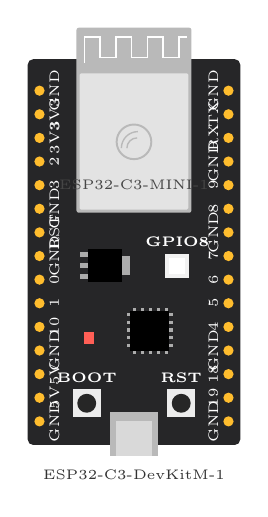
\begin{tikzpicture}
    \pic at (0,0) {esp32c3};
    \node[font=\tiny, text=gray!40!black, anchor=north] at (1.35,-0.2) {ESP32-C3-DevKitM-1};
  \end{tikzpicture}}

% ---------- Wokwi window (schematic; replace with a screenshot if you like) ----------
\newcommand{\wokwiwindow}{%
  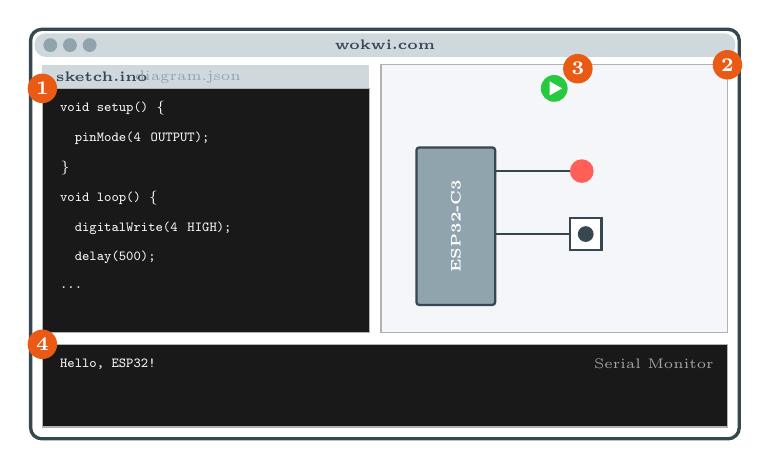
\begin{tikzpicture}[font=\tiny]
    \draw[nInk, very thick, fill=white, rounded corners=4pt] (0,0) rectangle (9,5.2);
    \fill[nLight, rounded corners=4pt] (0.05,4.85) rectangle (8.95,5.15);
    \fill[nLine] (0.25,5.0) circle (2.5pt); \fill[nLine] (0.5,5.0) circle (2.5pt); \fill[nLine] (0.75,5.0) circle (2.5pt);
    \node[font=\tiny\bfseries, text=nInk] at (4.5,5.0) {wokwi.com};
    % code editor
    \fill[nLight] (0.15,4.45) rectangle (4.3,4.75);
    \node[anchor=west, font=\tiny\bfseries, text=nInk] at (0.2,4.6) {sketch.ino};
    \node[anchor=west, font=\tiny, text=nLine] at (1.2,4.6) {diagram.json};
    \draw[gray!60, fill=VSDarkBg] (0.15,1.35) rectangle (4.3,4.45);
    \foreach \t [count=\j from 0] in {void setup() \{, \ \ pinMode(4\, OUTPUT);, \}, void loop() \{, \ \ digitalWrite(4\, HIGH);, \ \ delay(500);, \ldots}
      \node[anchor=west, text=VSText, font=\ttfamily\tiny] at (0.25,{4.2-0.38*\j}) {\t};
    % diagram
    \draw[gray!60, fill=LightGray] (4.45,1.35) rectangle (8.85,4.75);
    \fill[MacGreen] (6.65,4.45) circle (0.17);
    \fill[white] (6.59,4.36) -- (6.59,4.54) -- (6.75,4.45) -- cycle;
    \draw[nInk, thick, fill=nLine, rounded corners=1pt] (4.9,1.7) rectangle (5.9,3.7);
    \node[font=\tiny\bfseries, text=white, rotate=90] at (5.4,2.7) {ESP32-C3};
    \fill[MacRed] (7.0,3.4) circle (0.15);
    \draw[nInk, thick] (5.9,3.4) -- (6.85,3.4);
    \draw[nInk, thick, fill=white] (6.85,2.4) rectangle (7.25,2.8);
    \fill[nInk] (7.05,2.6) circle (0.1);
    \draw[nInk, thick] (5.9,2.6) -- (6.85,2.6);
    % serial monitor
    \draw[gray!60, fill=VSDarkBg] (0.15,0.15) rectangle (8.85,1.2);
    \node[anchor=west, text=VSText, font=\ttfamily\tiny] at (0.25,0.95) {Hello, ESP32!};
    \node[anchor=east, font=\tiny, text=gray!70] at (8.8,0.95) {Serial Monitor};
    % badges
    \foreach \x/\y/\n in {0.15/4.45/1, 8.85/4.75/2, 6.95/4.7/3, 0.15/1.2/4}
      \node[circle, fill=AccentOrange, text=white, font=\bfseries\scriptsize, inner sep=1.5pt] at (\x,\y) {\n};
  \end{tikzpicture}}

% ---------- our circuit for today ----------
\newcommand{\ourcircuit}{%
  \begin{tikzpicture}[>=Stealth, font=\scriptsize]
    \node[draw=nInk, very thick, fill=nInk, text=white, rounded corners=3pt, minimum width=2.0cm,
      minimum height=3.2cm, font=\scriptsize\bfseries, align=center] (esp) at (0,0) {ESP32-C3};
    \node[lbox, draw=nLine, fill=nFill, text=nInk, minimum width=1.9cm] (led) at (4.2,1.2) {\faLightbulb\ LED};
    \node[lbox, draw=nInk, fill=LightGray, minimum width=1.9cm] (ba) at (4.2,0.4) {\faDotCircle\ Button A};
    \node[lbox, draw=nInk, fill=LightGray, minimum width=1.9cm] (bb) at (4.2,-0.4) {\faDotCircle\ Button B};
    \node[lbox, draw=nLine, fill=nFill, text=nInk, minimum width=1.9cm] (lcd) at (4.2,-1.25) {\faTv\ LCD 16$\times$2};
    \draw[very thick, nInk] (esp.east |- led) -- node[above, font=\tiny] {GPIO 4} (led);
    \draw[very thick, nInk] (esp.east |- ba) -- node[above, font=\tiny] {GPIO 5} (ba);
    \draw[very thick, nInk] (esp.east |- bb) -- node[above, font=\tiny] {GPIO 6} (bb);
    \draw[very thick, nInk] (esp.east |- lcd) -- node[above, font=\tiny] {GPIO 8, 9 (I2C)} (lcd);
  \end{tikzpicture}}

% ---------- Wokwi-style parts for the "Build it" slides ----------
\definecolor{PcbBlack}{RGB}{38,38,40}
\definecolor{ResBody}{RGB}{214,184,140}
\definecolor{LcdScreen}{RGB}{131,190,40}
\definecolor{WireGreen}{RGB}{0,140,40}
\newcommand{\pinfont}{\fontsize{3.4}{3.6}\selectfont}
\tikzset{
  % a wire; the white edge makes crossings easy to see
  wire/.style={line width=1.1pt, rounded corners=1.5pt, preaction={draw, white, line width=2.6pt}},
  % ESP32-C3-DevKitM-1 as in Wokwi (USB at the bottom); pins (-L0)..(-L14), (-R0)..(-R14), 0 = top
  pics/esp32c3/.style={code={
    \fill[PcbBlack, rounded corners=2pt] (0,0) rectangle (2.7,4.9);
    % module ESP32-C3-MINI-1: the antenna part sticks out above the board
    \fill[gray!55, rounded corners=0.8pt] (0.62,2.95) rectangle (2.08,5.3);
    \draw[white, line width=0.5pt] (0.72,4.85) -- (0.72,5.18)
      \foreach \i in {1,...,3} { -- ++(0.2,0) -- ++(0,-0.26) -- ++(0.2,0) -- ++(0,0.26) } -- ++(0.1,0);
    \fill[gray!22, rounded corners=0.5pt] (0.66,2.99) rectangle (2.04,4.72);
    \draw[gray!55, line width=0.7pt] (1.35,3.85) circle (0.22);
    \draw[gray!55, line width=0.5pt] (1.26,3.77) arc (180:90:0.13) (1.19,3.77) arc (180:90:0.21);
    \node[font=\pinfont, text=gray!55!black] at (1.35,3.3) {ESP32-C3-MINI-1};
    % voltage regulator: 3 small legs on the left, a wide tab on the right
    \foreach \y in {2.14,2.28,2.42} \fill[gray!65] (0.66,\y-0.03) rectangle (0.76,\y+0.03);
    \fill[gray!65] (1.18,2.16) rectangle (1.3,2.4);
    \fill[black] (0.76,2.07) rectangle (1.2,2.49);
    % RGB LED on GPIO 8
    \fill[gray!10] (1.75,2.12) rectangle (2.05,2.42);
    \fill[white] (1.8,2.17) rectangle (2.0,2.37);
    \node[font=\pinfont\bfseries\rmfamily, text=white] at (1.9,2.58) {GPIO8};
    % USB-to-serial chip with pins on all sides
    \foreach \i in {0,...,4} {
      \fill[gray!65] ({1.34+0.1*\i},1.16) rectangle ++(0.04,0.05);
      \fill[gray!65] ({1.34+0.1*\i},1.69) rectangle ++(0.04,0.05);
      \fill[gray!65] (1.26,{1.24+0.1*\i}) rectangle ++(0.05,0.04);
      \fill[gray!65] (1.79,{1.24+0.1*\i}) rectangle ++(0.05,0.04);
    }
    \fill[black] (1.3,1.2) rectangle (1.8,1.7);
    % power LED
    \fill[MacRed] (0.72,1.28) rectangle (0.84,1.44);
    % BOOT and RST buttons
    \foreach \x/\t in {0.75/BOOT,1.95/RST} {
      \fill[gray!15] (\x-0.18,0.35) rectangle (\x+0.18,0.71);
      \fill[black!85] (\x,0.53) circle (0.12);
      \node[font=\pinfont\bfseries\rmfamily, text=white] at (\x,0.86) {\t};
    }
    % USB connector, sticks out below the board
    \fill[gray!55] (1.05,-0.14) rectangle (1.65,0.42);
    \fill[gray!30] (1.12,-0.14) rectangle (1.58,0.3);
    \foreach \n [count=\k from 0] in {GND,3V3,3V3,2,3,GND,RST,GND,0,1,10,GND,5V,5V,GND} {
      \fill[MacYellow] (0.15,{4.5-0.3*\k}) circle (0.065);
      \node[rotate=90, font=\pinfont, text=white] at (0.34,{4.5-0.3*\k}) {\n};
      \coordinate (-L\k) at (0.15,{4.5-0.3*\k});
    }
    \foreach \n [count=\k from 0] in {GND,TX,RX,GND,9,8,GND,7,6,5,4,GND,18,19,GND} {
      \fill[MacYellow] (2.55,{4.5-0.3*\k}) circle (0.065);
      \node[rotate=90, font=\pinfont, text=white] at (2.36,{4.5-0.3*\k}) {\n};
      \coordinate (-R\k) at (2.55,{4.5-0.3*\k});
    }
  }},
  % red LED, origin = middle of the rim; legs (-C) straight, (-A) bent
  pics/wled/.style={code={
    \draw[gray!60, line width=0.9pt] (-0.09,0) -- (-0.09,-0.42);
    \draw[gray!60, line width=0.9pt] (0.09,0) -- (0.09,-0.12) -- (0.17,-0.2) -- (0.17,-0.42);
    \fill[MacRed!80!black] (-0.24,0) rectangle (0.24,0.07);
    \fill[MacRed] (-0.2,0.07) -- (-0.2,0.32) arc (180:0:0.2) -- (0.2,0.07) -- cycle;
    \fill[white, opacity=0.45] (-0.1,0.38) ellipse (0.04 and 0.1);
    \node[font=\pinfont, text=black, anchor=east] at (-0.1,-0.3) {C};
    \node[font=\pinfont, text=black, anchor=west] at (0.18,-0.3) {A};
    \coordinate (-C) at (-0.09,-0.42);
    \coordinate (-A) at (0.17,-0.42);
  }},
  % 220 ohm resistor, vertical; origin = bottom lead (-2), top lead (-1)
  pics/wres/.style={code={
    \draw[gray!60, line width=0.9pt] (0,0) -- (0,0.85);
    \fill[ResBody, rounded corners=0.8pt] (-0.09,0.15) rectangle (0.09,0.7);
    \foreach \y/\c in {0.6/red, 0.52/red, 0.44/brown!80!black, 0.24/MacYellow!70!brown}
      \fill[\c] (-0.09,\y) rectangle (0.09,\y+0.05);
    \coordinate (-1) at (0,0.85);
    \coordinate (-2) at (0,0);
  }},
  % pushbutton, origin = centre; legs (-1l), (-2l), (-1r), (-2r); argument = colour of the cap
  pics/wbutton/.style={code={
    \foreach \x in {-1,1} \foreach \y in {-1,1}
      \draw[gray!60, line width=0.9pt] (0.3*\x,0.13*\y) -- (0.4*\x,0.13*\y);
    \fill[black!80, rounded corners=1pt] (-0.3,-0.25) rectangle (0.3,0.25);
    \fill[gray!35] (-0.25,-0.2) rectangle (0.25,0.2);
    \fill[#1] (0,0) circle (0.14);
    \node[font=\pinfont, text=black, anchor=south east] at (-0.33,0.13) {1.l};
    \node[font=\pinfont, text=black, anchor=north west] at (0.33,-0.13) {2.r};
    \node[font=\pinfont, text=black, anchor=north east] at (-0.33,-0.13) {2.l};
    \node[font=\pinfont, text=black, anchor=south west] at (0.33,0.13) {1.r};
    \coordinate (-1l) at (-0.4,0.13);  \coordinate (-2l) at (-0.4,-0.13);
    \coordinate (-1r) at (0.4,0.13);   \coordinate (-2r) at (0.4,-0.13);
  }},
  % LCD 16x2 with I2C, origin = bottom left; pins (-GND), (-VCC), (-SDA), (-SCL) on the left edge
  pics/wlcd/.style={code={
    \fill[mygreen!55!black, rounded corners=1.5pt] (0,0) rectangle (3.0,1.2);
    \fill[black!85] (0.55,0.12) rectangle (2.9,1.08);
    \fill[LcdScreen] (0.62,0.2) rectangle (2.83,1.0);
    \foreach \r in {0,1} \foreach \c in {0,...,15}
      \fill[LcdScreen!85!black] ({0.66+0.135*\c},{0.26+0.38*\r}) rectangle ++(0.11,0.3);
    \foreach \n [count=\k from 0] in {GND,VCC,SDA,SCL} {
      \fill[MacYellow] (0.14,{1.0-0.2*\k}) circle (0.055);
      \node[font=\pinfont, text=white, anchor=west] at (0.2,{1.0-0.2*\k}) {\n};
      \coordinate (-\n) at (0.14,{1.0-0.2*\k});
    }
  }},
}

% the circuit of the day, built in 4 steps: #1 = step (1 LED, 2 button A, 3 LCD, 4 button B)
% parts of the current step are drawn normally, parts of earlier steps are faded
\newcommand{\buildopacity}[2]{\ifnum#1>#2 0.3\else 1\fi}
\newcommand{\buildpic}[1]{%
  \begin{tikzpicture}[font=\tiny]
    \useasboundingbox (-0.45,-0.2) rectangle (7.3,5.7);
    \pic (esp) at (0,0) {esp32c3};
    % step 1: LED and resistor, GND along the bottom
    \begin{scope}[opacity=\buildopacity{#1}{1}]
      \pic (res) at (4.91,0.65) {wres};
      \pic (led) at (5.0,1.95) {wled};
      \draw[wire, black] (esp-R14) -- (4.91,0.3) -- (res-2);
      \draw[wire, WireGreen] (res-1) -- (led-C);
      \draw[wire, WireGreen] (esp-R10) -| (4.25,0.48) -| (led-A);
      \node[font=\fontsize{5.5}{6}\selectfont\bfseries, anchor=east] at (4.83,1.05) {220\,$\Omega$};
    \end{scope}
    % step 2: button A
    \ifnum#1>1
    \begin{scope}[opacity=\buildopacity{#1}{2}]
      \pic (ba) at (4.9,2.85) {wbutton=MacGreen};
      \node[font=\scriptsize\bfseries, anchor=south] at (4.9,3.1) {A};
      \draw[wire, black] (ba-2r) -| (5.75,0.3) -- (4.91,0.3);
      \draw[wire, WireGreen] (esp-R9) -| ([xshift=-0.35cm]ba-1l) -- (ba-1l);
    \end{scope}
    \fi
    % step 3: LCD (I2C)
    \ifnum#1>2
    \begin{scope}[opacity=\buildopacity{#1}{3}]
      \pic (lcd) at (4.2,4.2) {wlcd};
      \draw[wire, black] (esp-R0) -| ([xshift=-1.09cm]lcd-GND) -- (lcd-GND);
      \draw[wire, StorageBlue] (esp-R5) -| ([xshift=-0.59cm]lcd-SDA) -- (lcd-SDA);
      \draw[wire, ProgramPurple] (esp-R4) -| ([xshift=-0.79cm]lcd-SCL) -- (lcd-SCL);
      \draw[wire, MacRed] (esp-L12) -- (-0.35,0.9) -- (-0.35,5.6) -- (4.0,5.6) |- (lcd-VCC);
    \end{scope}
    \fi
    % step 4: button B
    \ifnum#1>3
    \begin{scope}[opacity=\buildopacity{#1}{4}]
      \pic (bb) at (4.9,3.75) {wbutton=StorageBlue};
      \node[font=\scriptsize\bfseries, anchor=south] at (4.9,4.0) {B};
      \draw[wire, black] (bb-2r) -| (5.75,2.72);
      \fill (5.75,2.72) circle (0.05);
      \draw[wire, WireGreen] (esp-R8) -| ([xshift=-0.55cm]bb-1l) -- (bb-1l);
    \end{scope}
    \fi
  \end{tikzpicture}}

% ---------- power: VCC, GND and a closed loop ----------
\newcommand{\powerexplain}{%
  \begin{tikzpicture}[font=\scriptsize, >=Stealth]
    % rails
    \draw[line width=2pt, nInk] (0,2.0) -- (4.6,2.0);
    \node[anchor=west, font=\scriptsize\bfseries, text=nInk, align=left] at (4.7,2.0) {VCC (+)\\[-1pt]{\tiny 3V3 = 3.3\,V, 5V = 5\,V}};
    \draw[line width=2pt, black] (0,-1.0) -- (4.6,-1.0);
    \node[anchor=west, font=\scriptsize\bfseries, align=left] at (4.7,-1.0) {GND ($-$)\\[-1pt]{\tiny 0\,V}};
    % voltage between the rails
    \draw[<->, thick, nInk] (-0.4,-1.0) -- node[left, font=\scriptsize\bfseries, align=center] {voltage\\3.3\,V} (-0.4,2.0);
    % a part between the rails: resistor + LED
    \draw[thick] (1.2,2.0) -- (1.2,1.55);
    \draw[thick, fill=ResBody] (1.08,1.55) rectangle (1.32,0.85);
    \draw[thick] (1.2,0.85) -- (1.2,0.6);
    \draw[thick, fill=nFill] (0.95,0.6) -- (1.45,0.6) -- (1.2,0.15) -- cycle;
    \draw[very thick] (0.95,0.15) -- (1.45,0.15);
    \foreach \d in {0,0.15} \draw[->, nInk, thick] (1.5,{0.45-\d}) -- ++(0.28,0.16);
    \draw[thick] (1.2,0.15) -- (1.2,-1.0);
    \fill[nInk] (1.2,2.0) circle (0.06);  \fill (1.2,-1.0) circle (0.06);
    \draw[->, line width=1.4pt, AccentOrange] (0.65,1.8) -- node[sloped, above, font=\tiny\bfseries] {current} (0.65,-0.8);
    \node[font=\tiny\bfseries, aExec, align=center] at (1.2,-1.4) {\faCheck\ closed loop:\\+ $\to$ part $\to$ GND};
    % a short circuit
    \draw[line width=1.4pt, aWrite] (3.6,2.0) -- (3.6,-1.0);
    \fill[nInk] (3.6,2.0) circle (0.06);  \fill (3.6,-1.0) circle (0.06);
    \node[font=\Large\bfseries, text=aWrite, fill=white, inner sep=1pt] at (3.6,0.5) {\faTimes};
    \node[font=\tiny\bfseries, aWrite, align=center] at (3.6,-1.4) {\faTimes\ short circuit:\\VCC straight to GND};
  \end{tikzpicture}}

% ---------- how an LED works: the part and its circuit ----------
\newcommand{\ledexplain}{%
  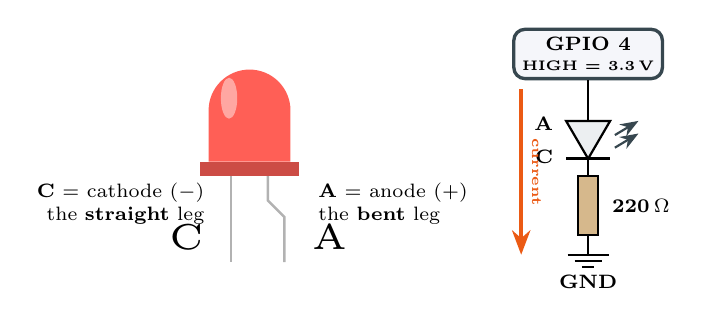
\begin{tikzpicture}[font=\scriptsize, >=Stealth]
    \begin{scope}[scale=2.6, transform shape]
      \pic (bl) at (0,0) {wled};
    \end{scope}
    \node[anchor=west, align=left] (la) at (0.75,-0.35) {\textbf{A} = anode (+)\\the \textbf{bent} leg};
    \node[anchor=east, align=right] (lc) at (-0.45,-0.35) {\textbf{C} = cathode ($-$)\\the \textbf{straight} leg};
    % the circuit
    \begin{scope}[xshift=4.3cm, yshift=-0.2cm]
      \node[lbox, draw=nInk, fill=LightGray] (gpio) at (0,1.75) {GPIO 4\\[-1pt]{\tiny HIGH = 3.3\,V}};
      \draw[thick] (gpio.south) -- (0,0.9);
      \draw[thick, fill=nFill] (-0.28,0.9) -- (0.28,0.9) -- (0,0.42) -- cycle;
      \draw[very thick] (-0.28,0.42) -- (0.28,0.42);
      \foreach \d in {0,0.16} \draw[->, nInk, thick] (0.34,{0.72-\d}) -- ++(0.3,0.18);
      \node[anchor=east, font=\scriptsize\bfseries] at (-0.32,0.86) {A};
      \node[anchor=east, font=\scriptsize\bfseries] at (-0.32,0.44) {C};
      \draw[thick] (0,0.42) -- (0,0.2);
      \draw[thick, fill=ResBody] (-0.13,0.2) rectangle (0.13,-0.55);
      \node[anchor=west, font=\scriptsize\bfseries] at (0.18,-0.18) {220\,$\Omega$};
      \draw[thick] (0,-0.55) -- (0,-0.8);
      \foreach \w/\y in {0.26/-0.8, 0.17/-0.88, 0.08/-0.96} \draw[thick] (-\w,\y) -- (\w,\y);
      \node[font=\scriptsize\bfseries] at (0,-1.15) {GND};
      \draw[->, line width=1.3pt, AccentOrange] (-0.85,1.3) -- node[sloped, above, font=\tiny\bfseries] {current} (-0.85,-0.8);
    \end{scope}
  \end{tikzpicture}}

% ---------- how a pushbutton works: 4 legs, 2 pairs ----------
% #1 = 0 not pressed, 1 pressed
\newcommand{\buttoninside}[1]{%
  \begin{tikzpicture}[font=\tiny, >=Stealth]
    \foreach \x/\y/\n in {0/0.8/1.l, 1.6/0.8/1.r, 0/0/2.l, 1.6/0/2.r} {
      \fill[gray!60] (\x,\y) circle (0.06);
      \node[font=\tiny\bfseries, anchor=\ifdim\x pt<1pt east\else west\fi] at (\x,\y) {\n};
    }
    \draw[thick] (0,0.8) -- (1.6,0.8);
    \draw[thick] (0,0) -- (1.6,0);
    \fill (0.8,0.8) circle (0.04);  \fill (0.8,0) circle (0.04);
    \ifnum#1=0
      \draw[thick] (0.8,0.8) -- (0.8,0.62) -- (1.1,0.22);
      \draw[thick] (0.8,0) -- (0.8,0.18);
    \else
      \draw[line width=1.6pt, nInk] (0.8,0.8) -- (0.8,0);
    \fi
  \end{tikzpicture}}
\newcommand{\buttonexplain}{%
  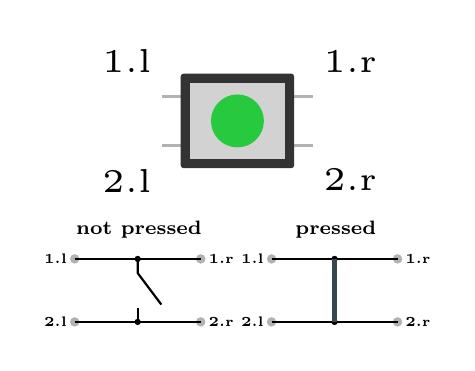
\begin{tikzpicture}[font=\scriptsize]
    \begin{scope}[scale=2.4, transform shape]
      \pic (bx) at (0,0) {wbutton=MacGreen};
    \end{scope}
    \node[anchor=north, align=center] at (-1.25,-1.15) {\textbf{not pressed}\\[2pt]\buttoninside{0}};
    \node[anchor=north, align=center] at (1.25,-1.15) {\textbf{pressed}\\[2pt]\buttoninside{1}};
  \end{tikzpicture}}

% ---------- I2C: one controller, many devices on 2 wires ----------
\newcommand{\itwocbus}{%
  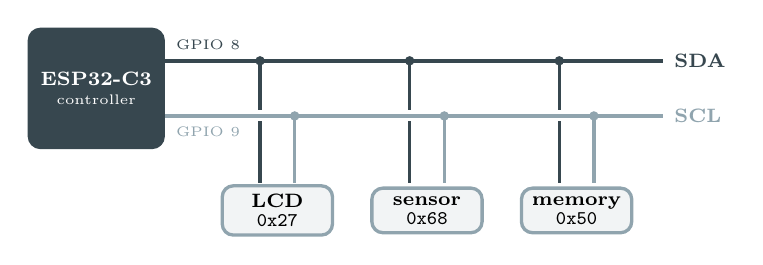
\begin{tikzpicture}[font=\scriptsize, >=Stealth]
    \node[lbox, draw=nInk, fill=nInk, text=white, minimum width=1.7cm, minimum height=1.5cm]
      (cpu) at (0,0) {ESP32-C3\\[-1pt]{\tiny\mdseries controller}};
    \draw[line width=1.5pt, nInk] (cpu.east |- 0,0.35) node[above right, font=\tiny] {GPIO 8} -- (7.2,0.35)
      node[right, font=\scriptsize\bfseries] {SDA};
    \foreach \x/\n/\a/\c in {2.3/LCD/0x27/nLine, 4.2/sensor/0x68/nLine, 6.1/memory/0x50/nLine} {
      \draw[line width=1.2pt, nInk] (\x-0.22,0.35) -- (\x-0.22,-1.2);
      \fill[nInk] (\x-0.22,0.35) circle (0.06);
      \node[lbox, draw=\c, fill=\c!12, minimum width=1.4cm] at (\x,-1.55) {\n\\[-1pt]\texttt{\a}};
    }
    \draw[line width=1.5pt, nLine, preaction={draw, white, line width=4pt}] (cpu.east |- 0,-0.35)
      node[below right, font=\tiny] {GPIO 9} -- (7.2,-0.35) node[right, font=\scriptsize\bfseries] {SCL};
    \foreach \x in {2.3,4.2,6.1} {
      \draw[line width=1.2pt, nLine] (\x+0.22,-0.35) -- (\x+0.22,-1.2);
      \fill[nLine] (\x+0.22,-0.35) circle (0.06);
    }
  \end{tikzpicture}}

% ---------- one I2C message on the wires: #1 = the step to highlight (1..6) ----------
\newcommand{\itwoctiming}[1]{%
  \begin{tikzpicture}[font=\scriptsize, >=Stealth]
    % the steps: highlighted band and a label on top
    \foreach \n/\a/\b/\t/\c in {1/0.3/1.0/START/AccentOrange, 2/1.0/5.0/{address \texttt{0x27} + write}/AccentOrange,
        3/5.0/5.5/ACK/AccentOrange, 4/5.5/9.5/{data byte}/AccentOrange, 5/9.5/10.0/ACK/AccentOrange, 6/10.0/10.75/STOP/AccentOrange} {
      \ifnum\n=#1
        \fill[\c!18, rounded corners=2pt] (\a,-1.55) rectangle (\b,1.45);
        \node[font=\scriptsize\bfseries, text=\c!80!black] at ({(\a+\b)/2},1.25) {\t};
      \else
        \node[font=\tiny, text=gray] at ({(\a+\b)/2},1.25) {\t};
      \fi
      \draw[gray!40, densely dotted] (\a,-1.55) -- (\a,1.1);
    }
    \node[anchor=east, font=\scriptsize\bfseries, text=nInk] at (-0.1,0.6) {SCL};
    \node[anchor=east, font=\scriptsize\bfseries, text=nInk] at (-0.1,-0.6) {SDA};
    % SCL: high, falls after START, 18 clock ticks, high again before STOP
    \draw[thick, nInk] (0,0.9) -- (0.8,0.9) -- (0.8,0.3) -- (1.25,0.3)
      \foreach \k in {0,...,17} { -- ({1.25+0.5*\k},0.9) -- ({1.5+0.5*\k},0.9) -- ({1.5+0.5*\k},0.3) -- ({1.75+0.5*\k},0.3) }
      -- (10.2,0.3) -- (10.2,0.9) -- (10.9,0.9);
    % SDA: falls at START, one bit per tick, rises at STOP
    \draw[thick, nInk] (0,-0.3) -- (0.5,-0.3) -- (0.5,-0.9) -- (1.0,-0.9);
    \foreach \x/\p/\v/\c in {1.0/0/0/nInk, 1.5/0/1/nInk, 2.0/1/0/nInk, 2.5/0/0/nInk, 3.0/0/1/nInk, 3.5/1/1/nInk, 4.0/1/1/nInk, 4.5/1/0/nInk, 5.0/0/0/nInk, 5.5/0/0/nInk, 6.0/0/1/nInk, 6.5/1/0/nInk, 7.0/0/0/nInk, 7.5/0/1/nInk, 8.0/1/0/nInk, 8.5/0/0/nInk, 9.0/0/0/nInk, 9.5/0/0/nInk}
      \draw[thick, \c] (\x,{-0.9+0.6*\p}) -- (\x,{-0.9+0.6*\v}) -- (\x+0.5,{-0.9+0.6*\v});
    \draw[thick, nInk] (10.0,-0.9) -- (10.45,-0.9) -- (10.45,-0.3) -- (10.9,-0.3);
    \foreach \x/\v in {1.25/0, 1.75/1, 2.25/0, 2.75/0, 3.25/1, 3.75/1, 4.25/1, 4.75/0, 5.25/0, 5.75/0, 6.25/1, 6.75/0, 7.25/0, 7.75/1, 8.25/0, 8.75/0, 9.25/0, 9.75/0} \node[font=\tiny, text=gray!70!black] at (\x,-1.2) {\v};
    \node[font=\tiny, text=gray!70!black] at (4.75,-1.42) {W};
  \end{tikzpicture}}

% ---------- showcase: Snake on a Nokia 5110 screen with a joystick ----------
\newcommand{\snakeshowcase}{%
  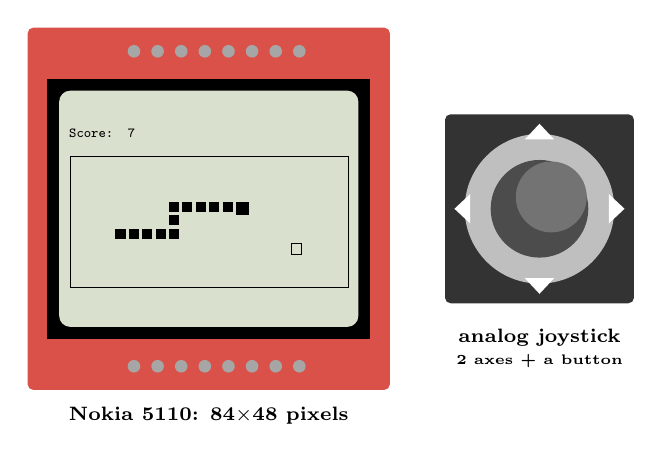
\begin{tikzpicture}[font=\scriptsize]
    % the Nokia 5110 module
    \fill[MacRed!85!black, rounded corners=2pt] (0,0) rectangle (4.6,4.6);
    \foreach \i in {0,...,7} {
      \fill[gray!70] ({1.35+0.3*\i},0.3) circle (0.08);
      \fill[gray!70] ({1.35+0.3*\i},4.3) circle (0.08);
    }
    \fill[black] (0.25,0.65) rectangle (4.35,3.95);
    \fill[LcdScreen!40!gray!30, rounded corners=4pt] (0.4,0.8) rectangle (4.2,3.8);
    % the game: 84 x 48 pixels drawn at 0.0425 cm per pixel
    \begin{scope}[shift={(0.52,3.32)}, x=0.0425cm, y=-0.0425cm]
      \node[anchor=north west, inner sep=0, font=\ttfamily\bfseries\tiny] at (0,0) {Score: 7};
      \draw[line width=0.3pt] (0.5,8.5) rectangle (83.5,47.5);
      \foreach \x/\y in {3/5,4/5,5/5,6/5,7/5,7/4,7/3,8/3,9/3,10/3,11/3} \fill ({2+4*\x},{10+4*\y}) rectangle ++(3,3);
      \fill ({2+4*12},{10+4*3}) rectangle ++(4,4);
      \draw[line width=0.3pt] ({2+4*16+0.5},{10+4*6+0.5}) rectangle ++(3,3);
    \end{scope}
    \node[font=\scriptsize\bfseries, anchor=north] at (2.3,-0.1) {Nokia 5110: 84$\times$48 pixels};
    % the joystick
    \begin{scope}[shift={(5.3,1.1)}]
      \fill[black!80, rounded corners=2pt] (0,0) rectangle (2.4,2.4);
      \fill[gray!50] (1.2,1.2) circle (0.95);
      \fill[black!70] (1.2,1.2) circle (0.62);
      \fill[black!55] (1.35,1.35) circle (0.45);
      \foreach \a in {0,90,180,270} \fill[white] ([shift={(\a:1.08)}]1.2,1.2) -- ([shift={(\a+12:0.9)}]1.2,1.2) -- ([shift={(\a-12:0.9)}]1.2,1.2) -- cycle;
      \node[font=\scriptsize\bfseries, anchor=north, align=center] at (1.2,-0.2) {analog joystick\\{\tiny 2 axes + a button}};
    \end{scope}
  \end{tikzpicture}}

% ---------- inside the ESP32-C3: CPU, internal bus, controllers; pins and wires outside ----------
% #1 = 0 overview, 1 address on the bus, 2 GPIO recognises it, 3 data written: the LED lights up
\newcommand{\chipbus}[1]{%
  \begin{tikzpicture}[>=Stealth, font=\scriptsize]
    % the chip
    \draw[nLine, very thick, dashed, rounded corners=6pt] (-1.3,-1.6) rectangle (11.9,2.5);
    \node[anchor=north west, font=\scriptsize\bfseries, text=nInk] at (-1.2,2.45) {\faMicrochip\ inside the ESP32-C3 chip};
    \node[cpubox, minimum width=1.8cm, minimum height=0.9cm] (cpu) at (0.4,1.45) {CPU};
    % the internal bus
    \ifnum#1>0 \def\buswidth{1.5pt}\else \def\buswidth{2pt}\fi
    \foreach \y/\c/\t in {0.75/nInk/address, 0.45/nLine/data, 0.15/nLight/control} {
      \draw[line width=\buswidth, \c] (0.4,\y) -- (10.4,\y);
      \node[anchor=west, font=\tiny\bfseries, text=\c] at (10.45,\y) {\t};
    }
    \node[font=\tiny\bfseries, text=nInk, anchor=south] at (5.4,0.78) {internal bus};
    \draw[very thick, nInk] (cpu.south) -- (0.4,0.15);
    % memory and controllers
    \node[rambox, minimum width=2.0cm, minimum height=0.85cm] (mem) at (2.9,-0.75) {Memory\\[-1pt]{\tiny\mdseries RAM, flash}};
    \node[iobox, minimum width=2.0cm, minimum height=0.85cm] (gpio) at (6.0,-0.75) {GPIO controller\\[-1pt]{\tiny\mdseries \texttt{0x6000\,4000}}};
    \node[iobox, minimum width=2.0cm, minimum height=0.85cm] (i2c) at (9.1,-0.75) {I2C controller\\[-1pt]{\tiny\mdseries \texttt{0x6001\,3000}}};
    \foreach \n in {mem,gpio,i2c} \draw[very thick, nInk] (\n.north) -- (\n.north |- 0,0.75);
    % every connection reaches all three groups of lines: address, data and control
    \foreach \x in {0.4,2.9,6.0,9.1}
      \foreach \y/\c in {0.75/nInk, 0.45/nLine, 0.15/nLight}
        \fill[\c] (\x,\y) circle (0.075);
    % pins on the edge of the chip, wires on the board
    \foreach \x/\l/\n in {5.6/4/gpio, 6.4/5/gpio, 8.7/8/i2c, 9.5/9/i2c} {
      \draw[thick, gray!70!black] (\x,-1.175) -- (\x,-1.6);
      \fill[MacYellow] (\x-0.09,-1.69) rectangle (\x+0.09,-1.51);
      \node[font=\tiny\bfseries, anchor=west] at (\x+0.08,-1.4) {\l};
    }
    \draw[line width=1.2pt, WireGreen] (5.6,-1.69) -- (5.6,-2.25);
    \draw[line width=1.2pt, WireGreen] (6.4,-1.69) -- (6.4,-2.25);
    \draw[line width=1.2pt, nInk] (8.7,-1.69) -- (8.7,-2.2);
    \draw[line width=1.2pt, nLine] (9.5,-1.69) -- (9.5,-2.2);
    \ifnum#1=3
      \fill[nLight] (5.6,-2.5) circle (0.38);
      \fill[nInk] (5.6,-2.5) circle (0.24);
      \node[font=\tiny\bfseries, text=nInk, anchor=east] at (5.5,-1.95) {3.3\,V};
    \else
      \fill[white] (5.6,-2.5) circle (0.24); \draw[nLine] (5.6,-2.5) circle (0.24);
    \fi
    \node[font=\tiny, anchor=north] at (5.6,-2.78) {LED};
    \fill[black!75, rounded corners=1pt] (6.2,-2.7) rectangle (6.6,-2.3);  \fill[MacGreen] (6.4,-2.5) circle (0.12);
    \node[font=\tiny, anchor=north] at (6.4,-2.78) {button};
    \node[lbox, draw=nLine, fill=nFill, text=nInk, minimum width=1.6cm] (lcd) at (9.1,-2.55) {LCD\\[-1pt]{\tiny\mdseries I2C address \texttt{0x27}}};
    \node[font=\tiny, text=gray!40!black, anchor=west, align=left] at (10.05,-1.95) {SDA, SCL:\\2 wires};
    \node[font=\scriptsize\bfseries, text=gray!40!black, anchor=west] at (-1.2,-2.2) {on the board: real wires};
    % the steps of one store: sw to 0x6000 4008
    \ifnum#1>0
      \node[font=\tiny\ttfamily, fill=white, draw=nInk, rounded corners=1pt, anchor=west] at (1.5,1.45) {sw a4, 8(a5)};
      \node[font=\tiny\bfseries\ttfamily, fill=white, draw=nLine, rounded corners=1pt] at (1.8,0.75) {0x6000\,4008};
    \fi
    \ifnum#1>1
      \draw[line width=1.6pt, AccentOrange, rounded corners=3pt] ([shift={(-0.08,-0.08)}]gpio.south west) rectangle ([shift={(0.08,0.08)}]gpio.north east);
      \node[font=\tiny\bfseries, text=AccentOrange, anchor=south west] at ([xshift=0.05cm]gpio.north east) {mine!};
      \node[font=\tiny, text=gray, anchor=south west] at ([xshift=0.05cm]mem.north east) {not mine};
      \node[font=\tiny, text=gray, anchor=south west] at ([xshift=0.05cm]i2c.north east) {not mine};
    \fi
    \ifnum#1>2
      \node[font=\tiny\bfseries\ttfamily, fill=white, draw=nLine, rounded corners=1pt] at (1.8,0.45) {0x10 = bit 4};
      \node[font=\tiny\bfseries, fill=white, awrite, rounded corners=1pt] at (1.8,0.15) {write};
    \fi
  \end{tikzpicture}}

% ---------- lcd.print: CPU -> I2C controller (internal bus) -> LCD (2 wires) ----------
\newcommand{\twobuses}{%
  \begin{tikzpicture}[>=Stealth, font=\scriptsize]
    \draw[nLine, very thick, dashed, rounded corners=6pt] (-0.3,-0.75) rectangle (5.3,1.2);
    \node[anchor=north west, font=\tiny\bfseries, text=nInk] at (-0.25,1.17) {\faMicrochip\ inside the chip};
    \node[cpubox, minimum width=1.4cm, minimum height=0.8cm] (cpu) at (0.6,0.1) {CPU};
    \node[iobox, minimum width=1.8cm, minimum height=0.8cm] (ctl) at (4.1,0.1) {I2C\\[-1pt]controller};
    \draw[->, line width=1.8pt, nInk] (cpu.east) -- node[above, font=\tiny\bfseries] {internal bus} node[below, font=\tiny\ttfamily] {sw \ldots\ 0x6001\,3xxx} (ctl.west);
    \node[lbox, draw=nLine, fill=nFill, text=nInk, minimum width=1.4cm, minimum height=0.8cm] (lcd) at (7.3,0.1) {LCD\\[-1pt]{\tiny\mdseries \texttt{0x27}}};
    \draw[->, line width=1.2pt, nInk] ([yshift=0.12cm]ctl.east) -- ([yshift=0.12cm]lcd.west);
    \draw[line width=1.2pt, nLine] ([yshift=-0.12cm]ctl.east) -- ([yshift=-0.12cm]lcd.west);
    \node[font=\tiny\bfseries, anchor=south] at (6.05,0.25) {SDA, SCL};
    \node[font=\tiny, anchor=north, align=center] at (6.05,-0.05) {START, \texttt{0x27},\\data, STOP};
    \node[font=\tiny\bfseries, text=gray!40!black] at (6.05,-0.95) {on the board};
    \node[font=\tiny\ttfamily, anchor=north] at (0.6,-0.32) {lcd.print("K")};
  \end{tikzpicture}}

% ---------- memory-mapped I/O: one address space, the device part zoomed in ----------
\newcommand{\mmiomap}{%
  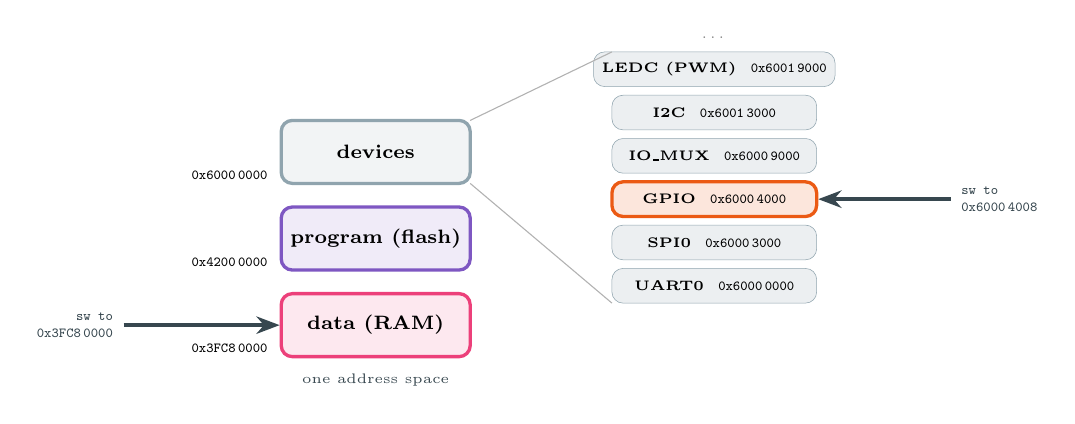
\begin{tikzpicture}[>=Stealth, font=\scriptsize]
    \foreach \y/\n/\a/\c in {2.3/devices/0x6000\,0000/nLine, 1.2/program (flash)/0x4200\,0000/sViolet, 0.1/data (RAM)/0x3FC8\,0000/sPink} {
      \node[lbox, draw=\c, fill=\c!12, minimum width=2.4cm, minimum height=0.8cm] (\n) at (0,\y) {\n};
      \node[font=\ttfamily\tiny, anchor=east] at (-1.25,\y-0.3) {\a};
    }
    \node[font=\tiny, text=nInk, anchor=north] at (0,-0.4) {one address space};
    % the device part, zoomed in: one window per controller
    \foreach \y/\n/\a/\h in {3.35/LEDC (PWM)/0x6001\,9000/0, 2.8/I2C/0x6001\,3000/0, 2.25/IO\_MUX/0x6000\,9000/0,
                             1.7/GPIO/0x6000\,4000/1, 1.15/SPI0/0x6000\,3000/0, 0.6/UART0/0x6000\,0000/0} {
      \ifnum\h=1
        \node[lbox, draw=AccentOrange, fill=AccentOrange!15, minimum width=2.6cm, minimum height=0.44cm, font=\tiny\bfseries] at (4.3,\y) {\n\ \ \texttt{\mdseries\a}};
      \else
        \node[lbox, draw=nLine, fill=nFill, minimum width=2.6cm, minimum height=0.44cm, font=\tiny\bfseries, very thin] at (4.3,\y) {\n\ \ \texttt{\mdseries\a}};
      \fi
    }
    \draw[gray!60, thin] (1.2,2.7) -- (3.0,3.57);
    \draw[gray!60, thin] (1.2,1.9) -- (3.0,0.38);
    \node[font=\tiny, text=gray] at (4.3,3.75) {\ldots};
    % two stores
    \draw[->, very thick, nInk] (7.3,1.7) node[right, font=\tiny\bfseries\ttfamily, align=left] {sw to\\0x6000\,4008} -- (5.62,1.7);
    \draw[->, very thick, nInk] (-3.2,0.1) node[left, font=\tiny\bfseries\ttfamily, align=right] {sw to\\0x3FC8\,0000} -- (-1.22,0.1);
  \end{tikzpicture}}

% ---------- small arrow "program flow" pieces ----------
\tikzset{
  instr/.style={draw=DeepBlue!60, fill=white, minimum width=1.9cm, minimum height=0.38cm, inner sep=1pt,
    font=\ttfamily\tiny},
  isrinstr/.style={instr, draw=cISR, fill=cISR!15},
}
\title{Computer Hardware}
\subtitle{Input/Output: Devices and Polling}
\author{Ksawery Możdżyński}
\date{}

% ---------- the course simulators: ksawerym.github.io/ComputerHardwareSimulators ----------
\newcommand{\simbase}{https://ksawerym.github.io/ComputerHardwareSimulators/}
\newcommand{\simlink}[1]{\href{\simbase\##1}{\texttt{ksawerym.github.io/ComputerHardwareSimulators/\##1}}}
% the address of a simulator topic, shown at the bottom of a slide
\newcommand{\simfoot}[1]{\par\vfill{\hfill\scriptsize\textcolor{gray}{\faLink\ #1}\par}}
% the same, in the title bar (for slides that are already full)
\newcommand{\simtop}[1]{\begin{tikzpicture}[remember picture,overlay]\node[anchor=east,inner sep=0pt,font=\scriptsize,text=white!80!nInk] at ([xshift=-0.35cm,yshift=-1.32cm]current page.north east) {\faLink\ #1};\end{tikzpicture}}

\begin{document}

\begin{frame}
  \titlepage
\end{frame}

\begin{frame}{Agenda For Today}
  \begin{columns}[T,onlytextwidth]
    \column{0.5\textwidth}
      \large
      \begin{itemize}
        \item[\textcolor{DeepBlue}{\faMicrochip}] \textbf{1. Meet the hardware} \\
        \textcolor{gray}{\small ESP32-C3 in Wokwi: LED, buttons, LCD}
      \end{itemize}
    \column{0.5\textwidth}
      \large
      \begin{itemize}
        \item[\textcolor{DeepBlue}{\faIcon{exchange-alt}}] \textbf{2. Talking to devices} \\
        \textcolor{gray}{\small Device registers and polling}
      \end{itemize}
  \end{columns}
\end{frame}

\begin{frame}{From last time: the CPU waits}
  \begin{beamercolorbox}[rounded=true,sep=0.12cm,wd=\textwidth]{block body}
    \centering\small The laptop CPU from last time: \textbf{3 GHz}, one cycle $\approx$ 0.3 ns.
  \end{beamercolorbox}
  \vspace{0.2cm}
  \begin{center}
    \footnotesize
    \renewcommand{\arraystretch}{1.25}
    \begin{tabular}{llrr}
      \toprule
      & \textbf{Waiting for} & \textbf{Time} & \textbf{Cycles} \\
      \midrule
      \textcolor{nInk}{\faMemory}  & main memory (last time) & 100 ns & about 300 \\
      \textcolor{cDisk}{\faHdd}     & a block from an SSD     & 50 $\mu$s & about 150\,000 \\
      \textcolor{cIO}{\faKeyboard}  & the next key you press  & 100 ms & about \textbf{300\,000\,000} \\
      \bottomrule
    \end{tabular}
  \end{center}
  \vfill
  \keymsg{Devices are \textbf{very} slow. Today: how the CPU talks to them without wasting its time.}
\end{frame}

% =====================================================================
\section{Meet the hardware}
% =====================================================================

\begin{frame}{Our computer for today: ESP32-C3}
  \begin{columns}[c,onlytextwidth]
    \column{0.35\textwidth}
      \centering
      \espboard
    \column{0.62\textwidth}
      \stepbox{\faMicrochip\ Processor}{\textbf{RISC-V}: the same instruction set as in Ripes. One core, up to 160 MHz.}
      \stepbox{\faMemory\ Memory}{400 KB of RAM on the chip.}
      \stepbox{\faPlug\ Input and output}{Pins (GPIO) for LEDs, buttons, displays and sensors.}
  \end{columns}
  \vfill
  \keymsg{A whole computer on one chip: CPU, memory and I/O.}
\end{frame}

\begin{frame}{Wokwi in one minute}
  \begin{columns}[c,onlytextwidth]
    \column{0.6\textwidth}
      \centering
      \resizebox{\linewidth}{!}{\wokwiwindow}
    \column{0.38\textwidth}
      \stepbox{\badge{1}\ Code}{The program (\texttt{sketch.ino}), in Arduino C++.}
      \stepbox{\badge{2}\ Diagram}{The board and the parts, connected with wires.}
      \stepbox{\badge{3}\ Run}{Compiles the program and starts the simulation.}
      \stepbox{\badge{4}\ Serial Monitor}{Text that the program prints.}
  \end{columns}
  \vfill
  \keymsg{Everything runs in the browser: nothing to install, nothing to break.}
\end{frame}

\begin{frame}{Power: VCC and GND}
  \begin{columns}[c,onlytextwidth]
    \column{0.55\textwidth}
      \centering
      \resizebox{\linewidth}{!}{\powerexplain}
    \column{0.43\textwidth}
      \stepbox{VCC (+)}{The supply: it pushes the current, like pressure in a pipe. Pins \textbf{3V3} and \textbf{5V}.}
      \stepbox{GND ($-$), ``ground''}{0\,V: every voltage is measured from here. All GND pins are connected together.}
      \stepbox{A closed loop}{Current flows only in a loop: from + through the part back to GND.}
      \stepbox{A GPIO pin}{\texttt{HIGH} = 3.3\,V, like VCC.\ \ \texttt{LOW} = 0\,V, like GND.}
  \end{columns}
  \vfill
  \keymsg{Never connect VCC straight to GND: that is a short circuit.}
\end{frame}

\begin{frame}{The LED: which leg goes where?}
  \begin{columns}[c,onlytextwidth]
    \column{0.55\textwidth}
      \centering
      \resizebox{\linewidth}{!}{\ledexplain}
    \column{0.43\textwidth}
      \stepbox{One way only}{Current flows only from \textbf{A} (+) to \textbf{C} ($-$).
        Turned around, the LED stays dark.}
      \stepbox{How to connect}{\textbf{A} $\to$ the GPIO pin.\ \ \textbf{C} $\to$ resistor $\to$ \textbf{GND}.}
      \stepbox{Why a resistor?}{It limits the current. Without it, a real LED (and the pin) can burn.}
      \stepbox{A real LED}{The \textbf{longer} leg is A. The flat edge of the case is on the C side.}
  \end{columns}
  \vfill
  \keymsg{GPIO 4 = HIGH: current flows A $\to$ C $\to$ resistor $\to$ GND, and the LED lights up.}
\end{frame}

\begin{frame}{Build it: the LED}
  \begin{columns}[c,onlytextwidth]
    \column{0.56\textwidth}
      \centering
      \resizebox{!}{0.72\textheight}{\buildpic{1}}
    \column{0.42\textwidth}
      \stepbox{\badge{1}\ Project}{wokwi.com: \textbf{ESP32} $\to$ Starter Templates $\to$ \textbf{ESP32-C3}.}
      \stepbox{\badge{2}\ Parts}{Click \textbf{+}, add an \textbf{LED} and a \textbf{Resistor} (220\,$\Omega$).}
      \stepbox{\badge{3}\ Wires}{Click a pin, then the other pin.
        GPIO \textbf{4} $\to$ LED \textsf{A} (the bent leg).
        LED \textsf{C} $\to$ resistor $\to$ \textbf{GND}.}
      \stepbox{\badge{4}\ Check}{Move the mouse over a pin to see its name.}
  \end{columns}
  \vfill
  \keymsg{Current flows from GPIO 4 through the LED and the resistor back to GND.}
\end{frame}

\begin{frame}[fragile]{Task 1: blink}
  \begin{columns}[T,onlytextwidth]
    \column{0.47\textwidth}
\begin{lstlisting}[style=ino]
#define LED 4

void setup() {
  pinMode(LED, OUTPUT);
}

void loop() {
  digitalWrite(LED, HIGH);   // on
  delay(@500@);                // wait 500 ms
  digitalWrite(LED, LOW);    // off
  delay(@500@);
}
\end{lstlisting}
    \column{0.5\textwidth}
      \taskhead{Task}{Open the project \textbf{Blink} from the course page.}
      {\scriptsize Or build it as on the previous slide: template \textbf{ESP32-C3}
        (not ESP32, -S3, -C6 or XIAO).\par}
      \vspace{0.1cm}
      \footnotesize
      \begin{enumerate}\setlength{\itemsep}{4pt}
        \item Press \textbf{Run} and watch the LED.
        \item Make the LED blink every \textbf{100 ms}.
        \item Make it blink \textbf{twice} quickly, then wait \textbf{1 second}, again and again.
      \end{enumerate}
      \vspace{0.1cm}
      \scriptsize\texttt{setup()} runs once at the start, \texttt{loop()} runs again and again.
  \end{columns}
\end{frame}

\begin{frame}[fragile]{Solution: blink}
  \begin{columns}[c,onlytextwidth]
    \column{0.5\textwidth}
\begin{lstlisting}[style=ino]
void loop() {
  for (int k = 0; k < 2; k++) {
    digitalWrite(LED, HIGH);
    delay(100);
    digitalWrite(LED, LOW);
    delay(100);
  }
  delay(1000);                // pause
}
\end{lstlisting}
    \column{0.46\textwidth}
      \stepbox{\texttt{pinMode}}{Pin 4 is an \textbf{output}: the program sets it.}
      \stepbox{\texttt{digitalWrite}}{\texttt{HIGH} = LED on, \texttt{LOW} = LED off.}
      \stepbox{\texttt{delay}}{The CPU waits and does \textbf{nothing else}. Remember this.}
  \end{columns}
\end{frame}

\begin{frame}{GPIO: pins the program controls}
  \begin{center}
    \begin{tikzpicture}[>=Stealth]
      \node[draw=nInk, very thick, fill=nInk, text=white, rounded corners=3pt, minimum width=2.2cm,
        minimum height=2.2cm, font=\small\bfseries] (esp) at (0,0) {ESP32-C3};
      \node[lbox, draw=nLine, fill=nFill, text=nInk, minimum width=2.4cm, minimum height=0.8cm] (led) at (-5.2,0) {\faLightbulb\ LED};
      \node[lbox, draw=nInk, fill=LightGray, minimum width=2.4cm, minimum height=0.8cm] (btn) at (5.2,0) {\faDotCircle\ Button};
      \draw[->, line width=2pt, nInk] (esp) -- node[above, font=\scriptsize\bfseries] {output} node[below, font=\tiny] {program writes 1 or 0} (led);
      \draw[->, line width=2pt, nInk] (btn) -- node[above, font=\scriptsize\bfseries] {input} node[below, font=\tiny] {program reads 1 or 0} (esp);
    \end{tikzpicture}
  \end{center}
  \vspace{0.2cm}
  \begin{columns}[T,onlytextwidth]
    \column{0.48\textwidth}
      \defbox{\textbf{GPIO} (General Purpose Input/Output): a pin that the program can \textbf{set} or \textbf{read}.}
    \column{0.48\textwidth}
      \stepbox{\texttt{INPUT\_PULLUP}}{The button pin reads \textbf{1} when not pressed, \textbf{0} when pressed.}
  \end{columns}
\end{frame}

\begin{frame}{The pushbutton: which legs to use?}
  \begin{columns}[c,onlytextwidth]
    \column{0.5\textwidth}
      \centering
      \resizebox{!}{0.62\textheight}{\buttonexplain}
    \column{0.48\textwidth}
      \stepbox{Four legs, two pairs}{\textsf{1.l} and \textsf{1.r} are \textbf{always} connected. So are \textsf{2.l} and \textsf{2.r}.}
      \stepbox{Pressing}{Connects pair \textbf{1} with pair \textbf{2}.}
      \stepbox{\ok\ Correct}{One wire on a \textbf{1} leg, the other on a \textbf{2} leg.
        We use \textsf{1.l} $\to$ GPIO 5 and \textsf{2.r} $\to$ GND.}
      \stepbox{\nok\ Wrong}{\textsf{1.l} and \textsf{1.r}: always connected. The pin always reads 0,
        as if the button were always pressed.}
  \end{columns}
\end{frame}

\begin{frame}[fragile]{Build it: add button A}
  \begin{columns}[c,onlytextwidth]
    \column{0.56\textwidth}
      \centering
      \resizebox{!}{0.72\textheight}{\buildpic{2}}
    \column{0.42\textwidth}
      \stepbox{\badge{1}\ Part}{Keep the LED. Click \textbf{+}, add a \textbf{Pushbutton}.}
      \stepbox{\badge{2}\ Wires}{GPIO \textbf{5} $\to$ button pin \textsf{1.l}.
        Button pin \textsf{2.r} $\to$ \textbf{GND}.}
      \stepbox{\badge{3}\ No bouncing}{In \texttt{diagram.json}, in the button's \texttt{attrs}, add:}
\begin{lstlisting}[style=term]
"bounce": "0"
\end{lstlisting}
  \end{columns}
  \vfill
  \keymsg{No resistor for the button: \texttt{INPUT\_PULLUP} gives the pin a 1 when the button is not pressed.}
\end{frame}

\begin{frame}[fragile]{Task 2: a button controls the LED}
  \begin{columns}[T,onlytextwidth]
    \column{0.5\textwidth}
\begin{lstlisting}[style=ino]
#define LED   4
#define BTN_A 5

void setup() {
  pinMode(LED, OUTPUT);
  pinMode(BTN_A, INPUT_PULLUP);
}

void loop() {
  // TODO: LED on only while
  //       the button is pressed
}
\end{lstlisting}
    \column{0.47\textwidth}
      \taskhead{Task}{Open the project \textbf{Button}. Complete \texttt{loop()}:
        the LED is on only while the button is pressed.}
      \footnotesize
      \texttt{digitalRead(BTN\_A)} gives \texttt{HIGH} or \texttt{LOW}.\\[0.1cm]
      In the simulation, click the button with the mouse and hold it.
  \end{columns}
\end{frame}

\begin{frame}[fragile]{Solution: a button controls the LED}
  \begin{columns}[c,onlytextwidth]
    \column{0.55\textwidth}
\begin{lstlisting}[style=ino]
void loop() {
  if (digitalRead(BTN_A) == LOW) {   // pressed
    digitalWrite(LED, HIGH);
  } else {                           // not pressed
    digitalWrite(LED, LOW);
  }
}
\end{lstlisting}
    \column{0.42\textwidth}
      \stepbox{Why \texttt{LOW}?}{With \texttt{INPUT\_PULLUP}, a pressed button connects the pin to ground: it reads \textbf{0}.}
      \stepbox{How often?}{\texttt{loop()} runs again and again, so the LED follows the button at once.}
  \end{columns}
\end{frame}

\begin{frame}[fragile]{The LCD 16$\times$2}
  \begin{columns}[c,onlytextwidth]
    \column{0.45\textwidth}
      \centering
      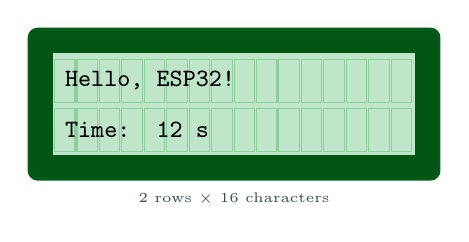
\begin{tikzpicture}
        \draw[mygreen!60!black, very thick, fill=mygreen!55!black, rounded corners=3pt] (0,0) rectangle (5.2,1.9);
        \fill[mygreen!25] (0.3,0.3) rectangle (4.9,1.6);
        \foreach \r in {0,1} \foreach \c in {0,...,15}
          \draw[mygreen!45] ({0.32+0.285*\c},{0.35+0.62*\r}) rectangle ++(0.26,0.55);
        \node[anchor=west, font=\ttfamily\small, text=black] at (0.33,1.25) {Hello, ESP32!};
        \node[anchor=west, font=\ttfamily\small, text=black] at (0.33,0.62) {Time: 12 s};
        \node[font=\tiny, text=nInk, anchor=north] at (2.6,-0.05) {2 rows $\times$ 16 characters};
      \end{tikzpicture}
    \column{0.52\textwidth}
\begin{lstlisting}[style=ino]
lcd.clear();              // empty screen
lcd.setCursor(0, 1);      // column 0, row 1
lcd.print("Time: ");      // text
lcd.print(12);            // or a number
\end{lstlisting}
      \vspace{0.1cm}
      \stepbox{Only 2 wires}{The LCD uses the \textbf{I2C bus}: 2 wires for all the data. How it works: after Task 3.}
  \end{columns}
\end{frame}

\begin{frame}{Build it: add the LCD}
  \begin{columns}[c,onlytextwidth]
    \column{0.56\textwidth}
      \centering
      \resizebox{!}{0.72\textheight}{\buildpic{3}}
    \column{0.42\textwidth}
      \stepbox{\badge{1}\ Part}{Click \textbf{+}, add an \textbf{LCD 16$\times$2 (I2C)}: it has only 4 pins.}
      \stepbox{\badge{2}\ Wires}{\textsf{SDA} $\to$ GPIO \textbf{8},\ \textsf{SCL} $\to$ GPIO \textbf{9},\\
        \textsf{VCC} $\to$ \textbf{5V},\ \textsf{GND} $\to$ \textbf{GND}.}
      \stepbox{\badge{3}\ Library}{Tab \textbf{Library Manager} $\to$ \textbf{+} $\to$ \texttt{LiquidCrystal I2C}.}
  \end{columns}
  \vfill
  \keymsg{I2C: data (\textsf{SDA}) and clock (\textsf{SCL}), plus power. The LCD's address is \texttt{0x27}.}
\end{frame}

\begin{frame}[fragile]{Task 3: hello, LCD}
  \begin{columns}[T,onlytextwidth]
    \column{0.52\textwidth}
\begin{lstlisting}[style=ino]
#include <Wire.h>              // I2C bus
#include <LiquidCrystal_I2C.h> // LCD over I2C

// address 0x27, 16 columns, 2 rows
LiquidCrystal_I2C lcd(0x27, 16, 2);

void setup() {
  Wire.begin(8, 9);  // I2C: SDA=8, SCL=9
  lcd.init();        // start the LCD
  lcd.backlight();   // light on
  // TODO 1
}

void loop() {
  // TODO 2
}
\end{lstlisting}
    \column{0.45\textwidth}
      \taskhead{Task}{Open the project \textbf{LCD}.}
      \footnotesize
      \begin{enumerate}\setlength{\itemsep}{4pt}
        \item \textbf{TODO 1}: show your name in \textbf{row 0}.
        \item \textbf{TODO 2}: show the number of \textbf{seconds} since the start in \textbf{row 1}.
      \end{enumerate}
      \vspace{0.1cm}
      \texttt{millis()} gives the time since the start in milliseconds.
  \end{columns}
\end{frame}

\begin{frame}[fragile]{Solution: hello, LCD}
  \begin{columns}[c,onlytextwidth]
    \column{0.52\textwidth}
\begin{lstlisting}[style=ino]
void setup() {
  Wire.begin(8, 9);           // I2C: SDA=8, SCL=9
  lcd.init();                 // start the LCD
  lcd.backlight();            // light on
  lcd.setCursor(0, 0);        // column 0, row 0
  lcd.print("Ksawery");       // TODO 1
}

void loop() {
  lcd.setCursor(0, 1);        // column 0, row 1
  lcd.print(millis() / 1000); // TODO 2: ms -> s
  lcd.print(" s");            // the unit
  delay(200);                 // wait 0.2 s
}
\end{lstlisting}
    \column{0.45\textwidth}
      \stepbox{Row 0}{Written once in \texttt{setup()}: it never changes.}
      \stepbox{Row 1}{Written again in every \texttt{loop()}, so the number keeps changing.}
      \stepbox{\texttt{delay(200)}}{Not needed for the result, but the LCD does not have to be redrawn thousands of times per second.}
  \end{columns}
\end{frame}

\begin{frame}{How I2C works}
  \begin{center}
    \resizebox{0.72\textwidth}{!}{\itwocbus}
  \end{center}
  \vspace{-0.1cm}
  \begin{columns}[T,onlytextwidth]
    \column{0.32\textwidth}
      \stepbox{\badge{1}\ Two wires}{\textsf{SCL}: the clock, given by the ESP32. \textsf{SDA}: one bit of data per clock tick.}
    \column{0.32\textwidth}
      \stepbox{\badge{2}\ Addresses}{Every device has its own address. The LCD is \texttt{0x27}: only it answers.}
    \column{0.32\textwidth}
      \stepbox{\badge{3}\ Messages}{Address first, then the data. Next slides: one message, step by step.}
  \end{columns}
\end{frame}

\begin{frame}{One I2C message, step by step\simtop{\simlink{io-i2c}}}
  \begin{center}
    \resizebox{\textwidth}{!}{%
      \only<1>{\itwoctiming{1}}%
      \only<2>{\itwoctiming{2}}%
      \only<3>{\itwoctiming{3}}%
      \only<4>{\itwoctiming{4}}%
      \only<5>{\itwoctiming{5}}%
      \only<6>{\itwoctiming{6}}%
    }
  \end{center}
  \vspace{-0.1cm}
  \only<1>{\stepbox{\badge{1}\ START\quad\textcolor{gray}{\mdseries(ESP32 $\to$ everyone)}}{SDA goes to 0 while SCL is 1. All devices wake up and listen: a message begins.}}
  \only<2>{\stepbox{\badge{2}\ Address + write\quad\textcolor{gray}{\mdseries(ESP32 $\to$ everyone)}}{7 address bits: \texttt{0x27} = \texttt{0100111}, one bit per SCL tick. Then 1 bit: \texttt{0} = write, \texttt{1} = read.}}
  \only<3>{\stepbox{\badge{3}\ ACK\quad\textcolor{gray}{\mdseries(LCD $\to$ ESP32)}}{Only the device with address \texttt{0x27} answers: it pulls SDA to 0 for the 9th tick: ``I am here, go on''. The others stay quiet.}}
  \only<4>{\stepbox{\badge{4}\ Data byte\quad\textcolor{gray}{\mdseries(ESP32 $\to$ LCD)}}{8 bits of data, e.g.\ a command or a piece of a letter for the screen.}}
  \only<5>{\stepbox{\badge{5}\ ACK\quad\textcolor{gray}{\mdseries(LCD $\to$ ESP32)}}{``Got it''. More bytes can follow, each one with its own ACK.}}
  \only<6>{\stepbox{\badge{6}\ STOP\quad\textcolor{gray}{\mdseries(ESP32 $\to$ everyone)}}{SDA goes to 1 while SCL is 1: the message is over, the bus is free again.}}
  \vfill
  \keymsg{Rule: SDA changes only while SCL is 0. A change while SCL is 1 means START or STOP.}
\end{frame}

\begin{frame}{Build it: add button B}
  \begin{columns}[c,onlytextwidth]
    \column{0.56\textwidth}
      \centering
      \resizebox{!}{0.72\textheight}{\buildpic{4}}
    \column{0.42\textwidth}
      \stepbox{\badge{1}\ Part}{A second \textbf{Pushbutton}: button B.}
      \stepbox{\badge{2}\ Wires}{GPIO \textbf{6} $\to$ pin \textsf{1.l}.
        Pin \textsf{2.r} $\to$ \textbf{GND}. Add \texttt{"bounce": "0"} here too.}
      \stepbox{\badge{3}\ Keep it}{Save the project: all later tasks use this circuit.}
  \end{columns}
  \vfill
  \keymsg{One GND pin can take many wires: all grounds are connected.}
\end{frame}

\begin{frame}[fragile]{Task 4: our circuit for today}
  \begin{columns}[c,onlytextwidth]
    \column{0.5\textwidth}
      \centering
      \ourcircuit
    \column{0.47\textwidth}
      \taskhead{Task}{Open the project \textbf{Circuit}. The program shows the state of both buttons.}
\begin{lstlisting}[style=ino]
lcd.setCursor(0, 0);
lcd.print("A:");
lcd.print(digitalRead(BTN_A));
lcd.print(" B:");
lcd.print(digitalRead(BTN_B));
\end{lstlisting}
      \footnotesize Run it. What does the LCD show when nothing is pressed? When you hold A? When you hold B?
  \end{columns}
\end{frame}

\begin{frame}{Solution: our circuit for today}
  \begin{columns}[c,onlytextwidth]
    \column{0.45\textwidth}
      \centering\footnotesize
      \renewcommand{\arraystretch}{1.25}
      \begin{tabular}{ll}
        \toprule
        \textbf{Part} & \textbf{Pin} \\
        \midrule
        LED & GPIO 4 \\
        Button A & GPIO 5 \\
        Button B & GPIO 6 \\
        LCD (SDA, SCL) & GPIO 8, 9 \\
        \bottomrule
      \end{tabular}
    \column{0.52\textwidth}
      \centering\footnotesize
      \renewcommand{\arraystretch}{1.25}
      \begin{tabular}{ll}
        \toprule
        \textbf{Buttons} & \textbf{LCD shows} \\
        \midrule
        nothing pressed & \texttt{A:1 B:1} \\
        A held          & \texttt{A:0 B:1} \\
        B held          & \texttt{A:1 B:0} \\
        \bottomrule
      \end{tabular}
  \end{columns}
  \vfill
  \keymsg{We keep this circuit for the whole day. Pressed = \textbf{0}, not pressed = \textbf{1}.}
\end{frame}

\begin{frame}{We can build real things with this}
  \begin{columns}[c,onlytextwidth]
    \column{0.55\textwidth}
      \centering
      \resizebox{\linewidth}{!}{\snakeshowcase}
    \column{0.43\textwidth}
      \stepbox{\faGamepad\ Snake}{The same ESP32-C3, a Nokia 5110 screen and a joystick: under 200 lines of code.}
      \stepbox{\faPlug\ Nothing new}{GPIO pins, a serial bus to the screen (SPI), analog inputs for the joystick,
        and \texttt{millis()} for the timing.}
      \stepbox{\faFolderOpen\ Try it}{The project \textbf{NokiaSnake} is on the course page.}
  \end{columns}
  \vfill
  \keymsg{Everything today works the same way on real hardware.}
\end{frame}

% =====================================================================
\section{Talking to devices}
% =====================================================================

\begin{frame}{How does the CPU reach a device?}
  \begin{center}
    \resizebox{!}{0.5\textheight}{\chipbus{0}}
  \end{center}
  \vspace{-0.15cm}
  \begin{columns}[T,onlytextwidth]
    \column{0.31\textwidth}
      \stepbox{Address lines}{\textbf{Who}: which memory cell or controller register.}
    \column{0.31\textwidth}
      \stepbox{Data lines}{\textbf{What}: the value to write or the value read.}
    \column{0.31\textwidth}
      \stepbox{Control lines}{\textbf{How}: read or write, and when.}
  \end{columns}
  \vfill
  \keymsg{The internal bus is \textbf{inside the chip}. The CPU talks only to \textbf{controllers}; they drive the pins.}
\end{frame}

\begin{frame}{One store to a device, step by step\simtop{\simlink{io-mmio}}}
  \begin{center}
    \resizebox{!}{0.52\textheight}{%
      \only<1>{\chipbus{1}}%
      \only<2>{\chipbus{2}}%
      \only<3>{\chipbus{3}}%
    }
  \end{center}
  \vspace{-0.15cm}
  \only<1>{\stepbox{\badge{1}\ Address}{The CPU runs \texttt{sw a4, 8(a5)} and puts the address \texttt{0x6000\,4008} on the
    address lines. Memory and every controller see it.}}
  \only<2>{\stepbox{\badge{2}\ Who is it for?}{Each one checks the address. \texttt{0x6000\,4xxx} belongs to the GPIO
    controller: \emph{mine!} Memory and the I2C controller ignore it.}}
  \only<3>{\stepbox{\badge{3}\ Data and write}{The CPU puts \texttt{0x10} (bit 4) on the data lines and \emph{write} on the
    control lines. The GPIO controller stores it: pin 4 goes to 3.3\,V and the LED lights up.}}
  \vfill
  \keymsg{The same \texttt{sw} as for memory. Only the \textbf{address} decides where the value goes.}
\end{frame}

\begin{frame}{Two buses, two kinds of address}
  \begin{center}
    \resizebox{0.62\textwidth}{!}{\twobuses}
  \end{center}
  \vspace{0.05cm}
  \begin{center}
    \footnotesize
    \renewcommand{\arraystretch}{1.2}
    \begin{tabular}{lll}
      \toprule
      & \textbf{Internal bus} & \textbf{I2C bus} \\
      \midrule
      Where          & inside the chip               & on the board \\
      Wires          & many, side by side            & 2: SDA and SCL \\
      An address is  & a \textbf{register}: \texttt{0x6000\,4008} & a \textbf{device}: \texttt{0x27} \\
      Speed          & a transfer in 1 clock cycle    & about 100\,000 bits per second \\
      \bottomrule
    \end{tabular}
  \end{center}
  \vfill
  \keymsg{\texttt{lcd.print}: the CPU writes to the I2C controller; the controller talks to the LCD over the 2 wires.}
\end{frame}

\begin{frame}{Memory-mapped I/O}
  \begin{columns}[c,onlytextwidth]
    \column{0.56\textwidth}
      \centering
      \resizebox{\linewidth}{!}{\mmiomap}
    \column{0.42\textwidth}
      \defbox{\textbf{Memory-mapped I/O}: the registers of every controller get addresses, just like memory cells.}
      \stepbox{A store to memory}{\texttt{sw} to \texttt{0x3FC8\,0000}: the value is saved in RAM.}
      \stepbox{A store to a device}{\texttt{sw} to \texttt{0x6000\,4008}: the value goes to the GPIO controller.}
      \stepbox{Fixed windows}{Every controller owns a range, set when the chip is designed. GPIO: \texttt{0x6000\,4000}--\texttt{4FFF}.}
  \end{columns}
  \vfill
  \keymsg{The same \texttt{sw} and \texttt{lw} from Ripes: the \textbf{address} decides whether it goes to memory or to a device.}
  \simfoot{\simlink{io-mmio}}
\end{frame}

\begin{frame}{The registers of the GPIO controller}
  \begin{center}
    \footnotesize
    \renewcommand{\arraystretch}{1.35}
    \begin{tabular}{@{}l l l l@{}}
      \toprule
      \textbf{Register} & \textbf{Address} & \textbf{Bit $n$ means \ldots} & \textbf{Used by} \\
      \midrule
      \texttt{ENABLE}   & \texttt{0x6000\,4020} & 1 = pin $n$ is an \textbf{output}, 0 = an input       & \texttt{pinMode} \\
      \texttt{OUT}      & \texttt{0x6000\,4004} & the level to \textbf{drive} on pin $n$: 1 = 3.3\,V, 0 = 0\,V & \\
      \texttt{OUT\_W1TS} & \texttt{0x6000\,4008} & write 1 $\to$ \textbf{set} bit $n$ of \texttt{OUT} (0 = no change)   & \texttt{digitalWrite(n, HIGH)} \\
      \texttt{OUT\_W1TC} & \texttt{0x6000\,400C} & write 1 $\to$ \textbf{clear} bit $n$ of \texttt{OUT} (0 = no change) & \texttt{digitalWrite(n, LOW)} \\
      \texttt{IN}       & \texttt{0x6000\,403C} & the level that \textbf{is} on pin $n$ now (read only)   & \texttt{digitalRead} \\
      \bottomrule
    \end{tabular}
  \end{center}
  \vspace{0.1cm}
  \begin{columns}[T,onlytextwidth]
    \column{0.48\textwidth}
      \stepbox{32 bits, one per pin}{In \textbf{every} register, bit $n$ is about pin GPIO $n$. Bit 4 is the LED, bit 5 is button A.}
    \column{0.48\textwidth}
      \stepbox{Why W1TS and W1TC?}{To change \textbf{one} pin with one \texttt{sw}. A write to \texttt{OUT} would change all 32 pins at once.}
  \end{columns}
  \simfoot{\simlink{io-gpio}}
\end{frame}

% GPIO register addresses checked in the ESP-IDF headers (soc/gpio_reg.h): W1TS 0x08, W1TC 0x0C, IN 0x3C.
\begin{frame}[fragile]{Task 5: an LED without \texttt{digitalWrite}}
  \begin{columns}[T,onlytextwidth]
    \column{0.55\textwidth}
\begin{lstlisting}[style=ino]
#define LED 4
#define GPIO_SET (*(volatile uint32_t *)0x60004008)
#define GPIO_CLR (*(volatile uint32_t *)0x6000400C)

void setup() {
  pinMode(LED, OUTPUT);
}

void loop() {
  @GPIO_SET = 1 << LED;@     // LED on
  delay(500);
  @GPIO_CLR = 1 << LED;@     // LED off
  delay(500);
}
\end{lstlisting}
    \column{0.42\textwidth}
      \taskhead{Task}{Open the project \textbf{Blink} from Task 1. Replace both \texttt{digitalWrite} lines
        with the two \textcolor{MacYellow!70!black}{\textbf{yellow}} lines.}
      \footnotesize
      \texttt{0x60004008}: write 1 to a bit $\rightarrow$ that pin goes \textbf{on}.\\
      \texttt{0x6000400C}: write 1 to a bit $\rightarrow$ that pin goes \textbf{off}.\\[0.1cm]
      Does the LED blink as in Task 1?
  \end{columns}
  \simfoot{\simlink{io-gpio}}
\end{frame}

\begin{frame}[fragile]{Solution: an LED without \texttt{digitalWrite}}
  \begin{columns}[c,onlytextwidth]
    \column{0.48\textwidth}
      {\scriptsize\textbf{C++}\par}
\begin{lstlisting}[style=ino]
GPIO_SET = 1 << LED;
\end{lstlisting}
      \vspace{0.1cm}
      {\scriptsize\textbf{What the compiler makes of it (RISC-V)}\par}
\begin{lstlisting}[style=rv]
lui  a5, 0x60004    # a5 = 0x60004000
li   a4, 16         # 1 << 4
sw   a4, 8(a5)      # store to 0x60004008
\end{lstlisting}
    \column{0.48\textwidth}
      \stepbox{Result}{The LED blinks exactly as in Task 1.}
      \stepbox{What happened}{One ordinary \texttt{sw}. Its address belongs to the GPIO device, not to RAM.}
      \stepbox{\texttt{volatile}}{Tells the compiler: \emph{really} do every access, this is a device.}
  \end{columns}
  \vfill
  \keymsg{For the CPU, a device is just a set of \textbf{addresses}.}
\end{frame}

\begin{frame}[fragile]{Task 6: read the button from its register}
  \begin{columns}[T,onlytextwidth]
    \column{0.55\textwidth}
\begin{lstlisting}[style=ino]
#define GPIO_IN (*(volatile uint32_t *)0x6000403C)

void loop() {
  uint32_t reg = GPIO_IN;         // one lw
  int a = @???@;                  // TODO: bit 5
  lcd.setCursor(0, 0);
  lcd.print("reg:");
  lcd.print(a);
  lcd.print(" dR:");
  lcd.print(digitalRead(BTN_A));
  delay(100);
}
\end{lstlisting}
    \column{0.42\textwidth}
      \taskhead{Task}{Open the project \textbf{Circuit}. The register at \texttt{0x6000403C} holds the state of
        \textbf{all} input pins: bit $n$ = pin $n$.}
      \footnotesize
      Complete the \texttt{TODO}: take bit \texttt{BTN\_A} (= 5) of \texttt{reg}.\\[0.1cm]
      Press A. Do \texttt{reg} and \texttt{dR} (\texttt{digitalRead}) always show the same value?\\[0.1cm]
      \scriptsize Hint: \texttt{(x >> n) \& 1} gives bit $n$ of \texttt{x}.
  \end{columns}
  \simfoot{\simlink{io-gpio}}
\end{frame}

\begin{frame}[fragile]{Solution: read the button from its register}
  \begin{columns}[c,onlytextwidth]
    \column{0.5\textwidth}
\begin{lstlisting}[style=ino]
int a = (reg >> BTN_A) & 1;
\end{lstlisting}
      \vspace{0.1cm}
      \centering
      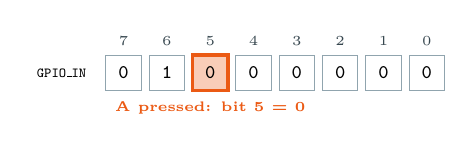
\begin{tikzpicture}
        \foreach \k/\v in {7/0,6/1,5/0,4/0,3/0,2/0,1/0,0/0} {
          \pgfmathsetmacro{\xx}{0.55*(7-\k)}
          \ifnum\k=5
            \node[draw=AccentOrange, very thick, fill=AccentOrange!30, minimum size=0.45cm, font=\ttfamily\scriptsize] at (\xx,0) {\v};
          \else
            \node[draw=nLine, fill=white, minimum size=0.45cm, font=\ttfamily\scriptsize] at (\xx,0) {\v};
          \fi
          \node[font=\tiny, text=nInk] at (\xx,0.4) {\k};
        }
        \node[font=\tiny, anchor=east] at (-0.35,0) {\texttt{GPIO\_IN}};
        \node[font=\tiny\bfseries, text=AccentOrange] at (1.1,-0.45) {A pressed: bit 5 = 0};
      \end{tikzpicture}
    \column{0.46\textwidth}
      \stepbox{Result}{\texttt{reg} and \texttt{dR} always agree: \texttt{digitalRead} reads the same register.}
      \stepbox{Status register}{This is the \textbf{status register} of the GPIO device: one bit per pin.}
  \end{columns}
  \vfill
  \keymsg{Reading a device = one \texttt{lw} from its status register.}
\end{frame}

\begin{frame}{Polling: asking again and again}
  \begin{columns}[c,onlytextwidth]
    \column{0.4\textwidth}
      \defbox{\textbf{Polling}: the CPU reads the status register again and again until something happens.}
      \stepbox{Like}{Checking your mailbox every minute, all day, to see if a letter came.}
    \column{0.57\textwidth}
      \centering
      \begin{tikzpicture}
        \tlbar{0}{CPU}{0.6/cPoll/?,0.6/cPoll/?,0.6/cPoll/?,0.6/cPoll/?,0.6/cPoll/?,0.6/cPoll/?,1.2/cWork/handle}
        \draw[->, thick, nInk] (0,-0.4) -- (5.0,-0.4) node[right, font=\tiny] {time};
        \node[font=\scriptsize\bfseries, text=cIO, anchor=south] at (3.9,0.3) {\faDotCircle\ pressed};
        \draw[cIO, very thick, dashed] (3.9,0.3) -- (3.9,-0.3);
      \end{tikzpicture}\\[0.2cm]
      \cpulegend
  \end{columns}
  \vfill
  \keymsg{Polling is simple: one loop. But what happens when the CPU also has other work?}
\end{frame}

\begin{frame}[fragile]{Task 7: polling can miss events}
  \begin{columns}[T,onlytextwidth]
    \column{0.52\textwidth}
\begin{lstlisting}[style=ino]
int count = 0;

void loop() {
  delay(2000);                    // "work": 2 s

  if (digitalRead(BTN_A) == LOW) { // check once
    count++;
  }
  lcd.setCursor(0, 1);
  lcd.print(count);
}
\end{lstlisting}
    \column{0.45\textwidth}
      \taskhead{Task}{Open the project \textbf{Polling}. The CPU works for 2 s, then checks the button once.}
      \footnotesize
      \begin{enumerate}\setlength{\itemsep}{4pt}
        \item Press button A \textbf{shortly} (click and release) \textbf{5 times} within about 10 seconds.
        \item Write down the number on the LCD.
      \end{enumerate}
  \end{columns}
  \simfoot{\simlink{cc-poll}}
\end{frame}

\begin{frame}{Solution: polling can miss events}
  \begin{center}
    \begin{tikzpicture}
      \tlbar{0}{CPU}{2.0/cWork/work,0.3/cPoll/?,2.0/cWork/work,0.3/cPoll/?,2.0/cWork/work,0.3/cPoll/?,2.0/cWork/work,0.3/cPoll/?}
      \foreach \x/\good in {0.9/0,2.25/1,3.4/0,5.6/0,7.5/0} {
        \node[font=\scriptsize, text=nInk] at (\x,0.55) {\faDotCircle};
        \node[font=\scriptsize, anchor=south, inner sep=1pt] at (\x,0.72) {\ifnum\good=1 \ok\else\nok\fi};
        \draw[nInk, thick, dashed] (\x,0.4) -- (\x,0.22);
      }
      \node[font=\tiny, text=nInk, anchor=west] at (9.3,0.55) {presses};
    \end{tikzpicture}\\[0.1cm]
    \cpulegend
  \end{center}
  \vspace{0.1cm}
  \begin{columns}[T,onlytextwidth]
    \column{0.48\textwidth}
      \stepbox{Result}{The LCD shows \textbf{fewer than 5}, often 0 or 1.}
    \column{0.48\textwidth}
      \stepbox{Why}{A press counts only if the button is held \textbf{exactly} when the CPU checks.
        A short click during the 2 s of work is lost.}
  \end{columns}
  \vfill
  \keymsg{While the CPU does other work, polling \textbf{misses} events.}
\end{frame}

\begin{frame}[fragile]{Task 8: polling wastes the CPU}
  \begin{columns}[T,onlytextwidth]
    \column{0.54\textwidth}
\begin{lstlisting}[style=ino]
uint32_t checks = 0, presses = 0;
int last = HIGH;

void loop() {
  int now = digitalRead(BTN_A);    // check
  checks++;
  if (last == HIGH && now == LOW) presses++;
  last = now;

  if (millis() >= 10000) {         // after 10 s
    lcd.setCursor(0, 0);
    lcd.print(checks);             // checks
    lcd.setCursor(0, 1);
    lcd.print(presses);            // presses
    while (true) { }               // stop
  }
}
\end{lstlisting}
    \column{0.43\textwidth}
      \taskhead{Task}{Open the project \textbf{Polling 2}. Now the CPU does \textbf{nothing} but check the button.}
      \footnotesize
      \begin{enumerate}\setlength{\itemsep}{4pt}
        \item Press A a few times within 10 s.
        \item Write down \textbf{checks} and \textbf{presses}.
        \item Compute: what percentage of the checks found a new press?
      \end{enumerate}
  \end{columns}
  \simfoot{\simlink{cc-poll}}
\end{frame}

\begin{frame}{Solution: polling wastes the CPU}
  \begin{columns}[c,onlytextwidth]
    \column{0.48\textwidth}
      \stepbox{Result}{Hundreds of thousands of checks, a handful of presses.\\[0.05cm]
        Example: 5 presses / 400\,000 checks = \textbf{0.00125\%}.}
      \stepbox{In other words}{More than \textbf{99.99\%} of the CPU's work was wasted.}
    \column{0.48\textwidth}
      \probbox{Your numbers}{Wokwi runs the CPU slower than the real chip, so you see fewer checks than a real ESP32-C3 would do.
        The conclusion does not change.}
  \end{columns}
  \vfill
  \keymsg{Polling \textbf{either} misses events (Task 7) \textbf{or} wastes the CPU (Task 8).}
\end{frame}

\end{document}